\documentclass{article}

\usepackage[margin = 0.7in]{geometry}
\usepackage{graphicx}
\usepackage{graphics}
\usepackage[T1]{fontenc}
\usepackage[polish]{babel}
\usepackage[utf8]{inputenc}
\usepackage{float}
\usepackage{tabularx}
\usepackage[table,xcdraw]{xcolor}
\usepackage{lipsum}
\usepackage{titlesec}
\usepackage{minted}
\usepackage{xcolor}

%TABS
\usepackage[]{booktabs}
\usepackage{tabularray}
\usepackage{multirow}


\title{Zadanie projektowe nr 1}
\author{Michał Dziedziak}
\date{\today}


\titlespacing\section{0pt}{12pt plus 4pt minus 2pt}{0pt plus 2pt minus 2pt}
\titlespacing\subsection{0pt}{12pt plus 4pt minus 2pt}{0pt plus 2pt minus 2pt}
\titlespacing\subsubsection{0pt}{12pt plus 4pt minus 2pt}{0pt plus 2pt minus 2pt}
\setlength{\parskip}{\baselineskip}%
\setlength{\parindent}{0pt}%

\newcommand{\squeezeup}{\vspace{-5mm}}


\begin{document}

\begin{titlepage}
    \begin{center}
        \vspace*{5cm}
        \rule{500pt}{1pt}\\
        \vspace*{0.5cm}
        \LARGE
        \textbf{Zadanie projektowe nr 1}\\
        \Large
        Badanie efektywności operacji dodawania, usuwania oraz wyszukiwania elementów \\
        w różnych strukturach danych\\
        \vspace*{0.5cm}
        \rule{500pt}{1pt}
    \end{center}

    \vspace*{12cm}

    {\raggedright
        \large
        \textbf{Autor sprawozdania:} Michał Dziedziak,  263901\\
        \textbf{Nazwisko i Imię prowadzącego kurs:} Mgr. inż. Antoni Sterna\\
        \textbf{Dzień i godzina zajęć:} Wtorek, 15:15 - 16:55 TN
    }
\end{titlepage}


\tableofcontents
\listoftables
\listoffigures


\newpage

%CONTENT
\section{Wstęp}
    \subsection{Zarys projektu}
    W ramach projektu w języku C++ zaimplementowane zostały wybrane struktury danych 
    i operacje z nimi związane. Poniższe sprawozdanie bada zależność czasu od ilości elementów w danych strukturach oraz porównuje to za teorią.

    \subsection{Struktury danych}
        \subsubsection{Zaimplementowane struktury i operacje}
        \begin{itemize}
            \item Tablica dynamiczna
            \begin{itemize}
                \item dodawanie na początek
                \item dodawanie na koniec
                \item dodawanie w wybrane miejsce
                \item usuwanie z początku
                \item usuwanie z końca
                \item usuwanie z wybranego miejsca
                \item szukanie elementu
            \end{itemize}
            \item Lista dwukierunkowa
            \begin{itemize}
                \item dodawanie na początek
                \item dodawanie na koniec
                \item dodawanie w wybrane miejsce
                \item usuwanie z początku
                \item usuwanie z końca
                \item usuwanie z wybranego miejsca
                \item szukanie elementu
            \end{itemize}
            \item Kopiec binarny
            \begin{itemize}
                \item dodawanie elementu
                \item usuwanie głowy
                \item szukanie elementu
            \end{itemize}
            \item Drzewo czerwono-czarne
            \begin{itemize}
                \item dodawanie elementu
                \item usuwanie elementu
                \item szukanie elementu
            \end{itemize}
        \end{itemize}

        \subsubsection{Teoretyczne złożoności obliczeniowe}
        W tej sekcji przedstawię teoretyczne złożoności obliczeniowe operacji na strukturach, celem późniejszego porównania ich z wynikami testów.
        \subsubsection{Złożoność obliczeniowa operacji w tablicy dynamicznej}
        \begin{center}    
            \begin{tabular}[H]{| c | c |}
                \hline
                Operacja & Średnia złożoność obliczeniowa \\ \hline \hline
                Dodanie elementu na początek & $O(n)$ \\ \hline
                Dodanie elementu na koniec & $O(n)$ \\ \hline
                Dodanie elementu w wybrane miejsce & $O(n)$ \\ \hline
                Usuwanie elementu z początku & $O(n)$ \\ \hline
                Usuwanie elementu z końca & $O(n)$ \\ \hline
                Usuwanie elementu z wybranego miejsca & $O(n)$ \\ \hline
                Szukanie elementu & $O(n)$ \\ \hline
            \end{tabular}
        \end{center}

        \subsubsection{Złożoność obliczeniowa operacji w liscie dwukierunkowej}
        \begin{center}    
            \begin{tabular}[H]{| c | c |}
                \hline
                Operacja & Średnia złożoność obliczeniowa \\ \hline \hline
                Dodanie elementu na początek & $O(1)$ \\ \hline
                Dodanie elementu na koniec & $O(1)$ \\ \hline
                Dodanie elementu w wybrane miejsce & $O(n)$ \\ \hline
                Usuwanie elementu z początku & $O(1)$ \\ \hline
                Usuwanie elementu z końca & $O(1)$ \\ \hline
                Usuwanie elementu z wybranego miejsca & $O(n)$ \\ \hline
                Szukanie elementu & $O(n)$ \\ \hline
            \end{tabular}
        \end{center}

        \subsubsection{Złożoność obliczeniowa operacji w kopcu binarnym}
        \begin{center}    
            \begin{tabular}[H]{| c | c |}
                \hline
                Operacja & Średnia złożoność obliczeniowa \\ \hline \hline
                Dodanie elementu & $O(\log n)$ \\ \hline
                Usunięcie głowy & $O(\log n)$ \\ \hline
                Szukanie elementu & $O(n)$ \\ \hline
            \end{tabular}
        \end{center}

        \subsubsection{Złożoność obliczeniowa operacji w drzewie czerwono-czarnym}
        \begin{center}    
            \begin{tabular}[H]{| c | c |}
                \hline
                Operacja & Średnia złożoność obliczeniowa \\ \hline \hline
                Dodanie elementu & $O(\log n)$ \\ \hline
                Usuwanie elementu & $O(\log n)$ \\ \hline
                Szukanie elementu & $O(\log n)$ \\ \hline
            \end{tabular}
        \end{center}
    
\section{Plan eksperymentu}
    \subsection{Założenia}
    \begin{itemize}
        \item Elementem każdej struktury jest 4 bajtowa liczba całkowita ze znakiem.
        \item Zakres (wielość) liczby będącej elementem zależy od ilości elementów w strukturze i jest równe przedziałowi od -<liczba elementów> do +<liczba elementów>
        \item Każda struktura jest alokowana dynamicznie, zajmując jak najmniej pamięci (miejsce w strukturach nie jest rezerwowane z zapasem). 
        \item Przeprowadzone testy badają zależność czasu od ilości elementów w strukturze. 
        \item Dla każdej operacji test powtarzany jest sto razy. Podczas każdej próby losowana jest nowa populacja, a ostateczny czas jest średnią czasów z prób.
        \item Testy rozpoczynają się dla 100000 elementów w strukturze i są zwiększane liniowo o 100000, aż do osiągnięcia 1000000 elementów.
        \item Dla każdego testu najpierw dodawana jest odpowiednia ilość elementów do struktury, a następnie mierzony jest czas wykonywania danej operacji.
    \end{itemize}

    \subsection{Pomiar czasu}
    Do pomiaru czasu została napisana osobna klasa "Timer". Korzysta ona z funkcji QueryPerformanceCounter\\
    i QueryPerformanceFrequency umożliwiających pomiar czasu z dokładnością do mikro sekund. Klasa ta określa upływ czasu, bazując na dokładnym liczniku.
    
    \subsection{Losowanie populacji}
    Do losowania populacji również została napisana osobna klasa RandomGenerator. Umożliwia ona losowanie pojedynczych liczb lub całych zbiorów.
    Korzysta z mt19937 - generatora liczb pseudolosowych.

\section{Zestawienie wyników}
    \subsection{Wyniki testów dla tablicy dynamicznej}
    \begin{table}[H]
        \centering
        \begin{tabular}{|c|ccc|}
            \hline
            \multirow{2}{*}{\textbf{Ilość   elementów}} & \multicolumn{3}{c|}{\textbf{Czas   potrzebny na wykonanie operacji {[}ms{]}}} \\ \cline{2-4} 
             & \multicolumn{1}{c|}{\textbf{Dodaj na początek}} & \multicolumn{1}{c|}{\textbf{Dodaj na koniec}} & \textbf{Dodaj w wybrane   miejsce} \\ \hline
            100000 & \multicolumn{1}{c|}{0.31} & \multicolumn{1}{c|}{0.27} & 0.28 \\ \hline
            200000 & \multicolumn{1}{c|}{0.69} & \multicolumn{1}{c|}{0.60} & 0.69 \\ \hline
            300000 & \multicolumn{1}{c|}{1.18} & \multicolumn{1}{c|}{1.30} & 1.17 \\ \hline
            400000 & \multicolumn{1}{c|}{1.46} & \multicolumn{1}{c|}{1.63} & 1.46 \\ \hline
            500000 & \multicolumn{1}{c|}{1.79} & \multicolumn{1}{c|}{2.20} & 1.99 \\ \hline
            600000 & \multicolumn{1}{c|}{2.14} & \multicolumn{1}{c|}{2.19} & 2.27 \\ \hline
            700000 & \multicolumn{1}{c|}{2.33} & \multicolumn{1}{c|}{2.30} & 2.33 \\ \hline
            800000 & \multicolumn{1}{c|}{2.83} & \multicolumn{1}{c|}{2.98} & 3.05 \\ \hline
            900000 & \multicolumn{1}{c|}{3.01} & \multicolumn{1}{c|}{2.94} & 3.41 \\ \hline
            1000000 & \multicolumn{1}{c|}{3.70} & \multicolumn{1}{c|}{3.34} & 3.66 \\ \hline
        \end{tabular}
        \caption{Pomiary tablicy dynamicznej 1/2}
        % \label{tab:my-table}
    \end{table}

    
    \begin{table}[H]
        \centering
        \begin{tabular}{|c|cccc|}
            \hline
            \multirow{2}{*}{\textbf{Ilość   elementów}} & \multicolumn{4}{c|}{\textbf{Czas potrzebny na wykonanie operacji {[}ms{]}}} \\ \cline{2-5} 
             & \multicolumn{1}{c|}{\textbf{Usuń z początku}} & \multicolumn{1}{c|}{\textbf{Usuń z końca}} & \multicolumn{1}{c|}{\textbf{Usuń z wybranego   miejsca}} & \textbf{Znajdź element} \\ \hline
            100000 & \multicolumn{1}{c|}{0.25} & \multicolumn{1}{c|}{0.26} & \multicolumn{1}{c|}{0.25} & 0.20 \\ \hline
            200000 & \multicolumn{1}{c|}{0.66} & \multicolumn{1}{c|}{0.62} & \multicolumn{1}{c|}{0.62} & 0.30 \\ \hline
            300000 & \multicolumn{1}{c|}{1.02} & \multicolumn{1}{c|}{1.18} & \multicolumn{1}{c|}{1.13} & 0.51 \\ \hline
            400000 & \multicolumn{1}{c|}{1.57} & \multicolumn{1}{c|}{1.46} & \multicolumn{1}{c|}{1.30} & 0.67 \\ \hline
            500000 & \multicolumn{1}{c|}{1.92} & \multicolumn{1}{c|}{1.84} & \multicolumn{1}{c|}{1.63} & 0.83 \\ \hline
            600000 & \multicolumn{1}{c|}{2.15} & \multicolumn{1}{c|}{2.05} & \multicolumn{1}{c|}{1.95} & 1.01 \\ \hline
            700000 & \multicolumn{1}{c|}{2.63} & \multicolumn{1}{c|}{2.41} & \multicolumn{1}{c|}{2.52} & 1.37 \\ \hline
            800000 & \multicolumn{1}{c|}{2.56} & \multicolumn{1}{c|}{2.66} & \multicolumn{1}{c|}{2.86} & 1.53 \\ \hline
            900000 & \multicolumn{1}{c|}{3.17} & \multicolumn{1}{c|}{3.04} & \multicolumn{1}{c|}{3.23} & 1.47 \\ \hline
            1000000 & \multicolumn{1}{c|}{3.71} & \multicolumn{1}{c|}{3.49} & \multicolumn{1}{c|}{3.54} & 1.82 \\ \hline
        \end{tabular}
        \caption{Pomiary tablicy dynamicznej 2/2}
        % \label{tab:my-table}
    \end{table}


    \begin{figure}[H]
        \centering
        \includegraphics[scale = 0.85]{wykresy/arr/addFirst.png}
        \caption{Wykres czasu od ilości elementów dla Tablicy - dodaj na początek}
    \end{figure}

    \begin{figure}[H]
        \centering
        \includegraphics[scale = 0.85]{wykresy/arr/addLast.png}
        \caption{Wykres czasu od ilości elementów dla Tablicy - dodaj na koniec}
    \end{figure}

    \begin{figure}[H]
        \centering
        \includegraphics[scale = 0.85]{wykresy/arr/addIndex.png}
        \caption{Wykres czasu od ilości elementów dla Tablicy - dodaj w wybrane miejsce}
    \end{figure}

    \begin{figure}[H]
        \centering
        \includegraphics[scale = 0.85]{wykresy/arr/removeFirst.png}
        \caption{Wykres czasu od ilości elementów dla Tablicy - usuń z początku}
    \end{figure}

    
    \begin{figure}[H]
        \centering
        \includegraphics[scale = 0.85]{wykresy/arr/removeLast.png}
        \caption{Wykres czasu od ilości elementów dla Tablicy - usuń z końca}
    \end{figure}
    
    \begin{figure}[H]
        \centering
        \includegraphics[scale = 0.85]{wykresy/arr/removeIndex.png}
        \caption{Wykres czasu od ilości elementów dla Tablicy - usuń z wybranego miejsca}
    \end{figure}
    
    \begin{figure}[H]
        \centering
        \includegraphics[scale = 0.85]{wykresy/arr/find.png}
        \caption{Wykres czasu od ilości elementów dla Tablicy - znajdź element}
    \end{figure}    


    \subsection{Wyniki testów dla listy dwukierunkowej}
    \begin{table}[H]
        \centering
        \begin{tabular}{|c|cccc|}
            \hline
            \multirow{2}{*}{\textbf{Ilość   elementów}} & \multicolumn{4}{c|}{\textbf{Czas   potrzebny na wykonanie operacji {[}us{]}}} \\ \cline{2-5} 
             & \multicolumn{1}{c|}{\textbf{Dodaj na początek}} & \multicolumn{1}{c|}{\textbf{Dodaj na koniec}} & \multicolumn{1}{c|}{\textbf{Usuń z początku}} & \textbf{Usuń z końca} \\ \hline
            100000 & \multicolumn{1}{c|}{0.11} & \multicolumn{1}{c|}{0.08} & \multicolumn{1}{c|}{0.72} & 0.52 \\ \hline
            200000 & \multicolumn{1}{c|}{0.14} & \multicolumn{1}{c|}{0.10} & \multicolumn{1}{c|}{0.74} & 0.56 \\ \hline
            300000 & \multicolumn{1}{c|}{0.13} & \multicolumn{1}{c|}{0.10} & \multicolumn{1}{c|}{0.81} & 0.50 \\ \hline
            400000 & \multicolumn{1}{c|}{0.12} & \multicolumn{1}{c|}{0.13} & \multicolumn{1}{c|}{0.89} & 0.50 \\ \hline
            500000 & \multicolumn{1}{c|}{0.14} & \multicolumn{1}{c|}{0.11} & \multicolumn{1}{c|}{0.74} & 0.47 \\ \hline
            600000 & \multicolumn{1}{c|}{0.11} & \multicolumn{1}{c|}{0.10} & \multicolumn{1}{c|}{0.73} & 0.46 \\ \hline
            700000 & \multicolumn{1}{c|}{0.12} & \multicolumn{1}{c|}{0.09} & \multicolumn{1}{c|}{0.63} & 0.49 \\ \hline
            800000 & \multicolumn{1}{c|}{0.12} & \multicolumn{1}{c|}{0.09} & \multicolumn{1}{c|}{0.66} & 0.48 \\ \hline
            900000 & \multicolumn{1}{c|}{0.12} & \multicolumn{1}{c|}{0.09} & \multicolumn{1}{c|}{0.65} & 0.49 \\ \hline
            1000000 & \multicolumn{1}{c|}{0.12} & \multicolumn{1}{c|}{0.09} & \multicolumn{1}{c|}{0.66} & 0.46 \\ \hline
        \end{tabular}
        \caption{Pomiary listy dwukierunkowej 1/2}
        % \label{tab:my-table}
    \end{table}

    \begin{table}[H]
        \centering
        \begin{tabular}{|c|ccc|}
            \hline
            \multirow{2}{*}{\textbf{Ilość   elementów}} & \multicolumn{3}{c|}{\textbf{Czas   potrzebny na wykonanie operacji {[}us{]}}} \\ \cline{2-4} 
             & \multicolumn{1}{c|}{\textbf{Dodaj w wybrane miejsce}} & \multicolumn{1}{c|}{\textbf{Usuń z wybranego   miejsca}} & \textbf{Znajdź element} \\ \hline
            100000 & \multicolumn{1}{c|}{0.23} & \multicolumn{1}{c|}{0.26} & 0.72 \\ \hline
            200000 & \multicolumn{1}{c|}{0.49} & \multicolumn{1}{c|}{0.50} & 1.40 \\ \hline
            300000 & \multicolumn{1}{c|}{0.69} & \multicolumn{1}{c|}{0.77} & 2.07 \\ \hline
            400000 & \multicolumn{1}{c|}{0.97} & \multicolumn{1}{c|}{1.16} & 2.44 \\ \hline
            500000 & \multicolumn{1}{c|}{1.33} & \multicolumn{1}{c|}{1.21} & 3.47 \\ \hline
            600000 & \multicolumn{1}{c|}{1.70} & \multicolumn{1}{c|}{1.61} & 4.62 \\ \hline
            700000 & \multicolumn{1}{c|}{1.76} & \multicolumn{1}{c|}{1.85} & 4.75 \\ \hline
            800000 & \multicolumn{1}{c|}{2.20} & \multicolumn{1}{c|}{2.11} & 5.70 \\ \hline
            900000 & \multicolumn{1}{c|}{2.15} & \multicolumn{1}{c|}{2.22} & 6.19 \\ \hline
            1000000 & \multicolumn{1}{c|}{2.72} & \multicolumn{1}{c|}{2.47} & 6.94 \\ \hline
        \end{tabular}
        \caption{Pomiary listy dwukierunkowej 2/2}
        % \label{tab:my-table}
    \end{table}


    \begin{figure}[H]
        \centering
        \includegraphics[scale = 0.85]{wykresy/table/addFirst.png}
        \caption{Wykres czasu od ilości elementów dla Listy - dodaj na początek}
    \end{figure}

    \begin{figure}[H]
        \centering
        \includegraphics[scale = 0.85]{wykresy/table/addLast.png}
        \caption{Wykres czasu od ilości elementów dla Listy - dodaj na koniec}
    \end{figure}

    \begin{figure}[H]
        \centering
        \includegraphics[scale = 0.85]{wykresy/table/addIndex.png}
        \caption{Wykres czasu od ilości elementów dla Listy - dodaj w wybrane miejsce}
    \end{figure}

    \begin{figure}[H]
        \centering
        \includegraphics[scale = 0.85]{wykresy/table/removeFirst.png}
        \caption{Wykres czasu od ilości elementów dla Listy - usuń z początku}
    \end{figure}

    
    \begin{figure}[H]
        \centering
        \includegraphics[scale = 0.85]{wykresy/table/removeLast.png}
        \caption{Wykres czasu od ilości elementów dla Listy - usuń z końca}
    \end{figure}
    
    \begin{figure}[H]
        \centering
        \includegraphics[scale = 0.85]{wykresy/table/removeIndex.png}
        \caption{Wykres czasu od ilości elementów dla Listy - usuń z wybranego miejsca}
    \end{figure}
    
    \begin{figure}[H]
        \centering
        \includegraphics[scale = 0.85]{wykresy/table/find.png}
        \caption{Wykres czasu od ilości elementów dla Listy - znajdź element}
    \end{figure}  


    \subsection{Wyniki testów dla kopca binarnego}
    \begin{table}[H]
        \centering
        \begin{tabular}{|c|ccc|}
            \hline
            \multirow{2}{*}{\textbf{Ilość   elementów}} & \multicolumn{3}{c|}{\textbf{Czas   potrzebny na wykonanie operacji {[}ms{]}}} \\ \cline{2-4} 
             & \multicolumn{1}{c|}{\textbf{Dodaj element}} & \multicolumn{1}{c|}{\textbf{Usuń element z głowy}} & \textbf{Znajdź element} \\ \hline
            100000 & \multicolumn{1}{c|}{0.27} & \multicolumn{1}{c|}{0.26} & 0.15 \\ \hline
            200000 & \multicolumn{1}{c|}{0.43} & \multicolumn{1}{c|}{0.52} & 0.35 \\ \hline
            300000 & \multicolumn{1}{c|}{0.87} & \multicolumn{1}{c|}{0.86} & 0.45 \\ \hline
            400000 & \multicolumn{1}{c|}{1.29} & \multicolumn{1}{c|}{1.30} & 0.63 \\ \hline
            500000 & \multicolumn{1}{c|}{1.68} & \multicolumn{1}{c|}{1.48} & 0.88 \\ \hline
            600000 & \multicolumn{1}{c|}{1.90} & \multicolumn{1}{c|}{1.75} & 1.05 \\ \hline
            700000 & \multicolumn{1}{c|}{2.17} & \multicolumn{1}{c|}{2.20} & 1.28 \\ \hline
            800000 & \multicolumn{1}{c|}{2.51} & \multicolumn{1}{c|}{2.40} & 1.55 \\ \hline
            900000 & \multicolumn{1}{c|}{2.94} & \multicolumn{1}{c|}{2.84} & 1.48 \\ \hline
            1000000 & \multicolumn{1}{c|}{3.03} & \multicolumn{1}{c|}{3.02} & 1.82 \\ \hline
        \end{tabular}
        \caption{Pomiary kopca binarnego}
        % \label{tab:my-table}
    \end{table}


    
    \begin{figure}[H]
        \centering
        \includegraphics[scale = 0.85]{wykresy/heap/add.png}
        \caption{Wykres czasu od ilości elementów dla Kopca - dodaj element (push)}
    \end{figure}
    
    \begin{figure}[H]
        \centering
        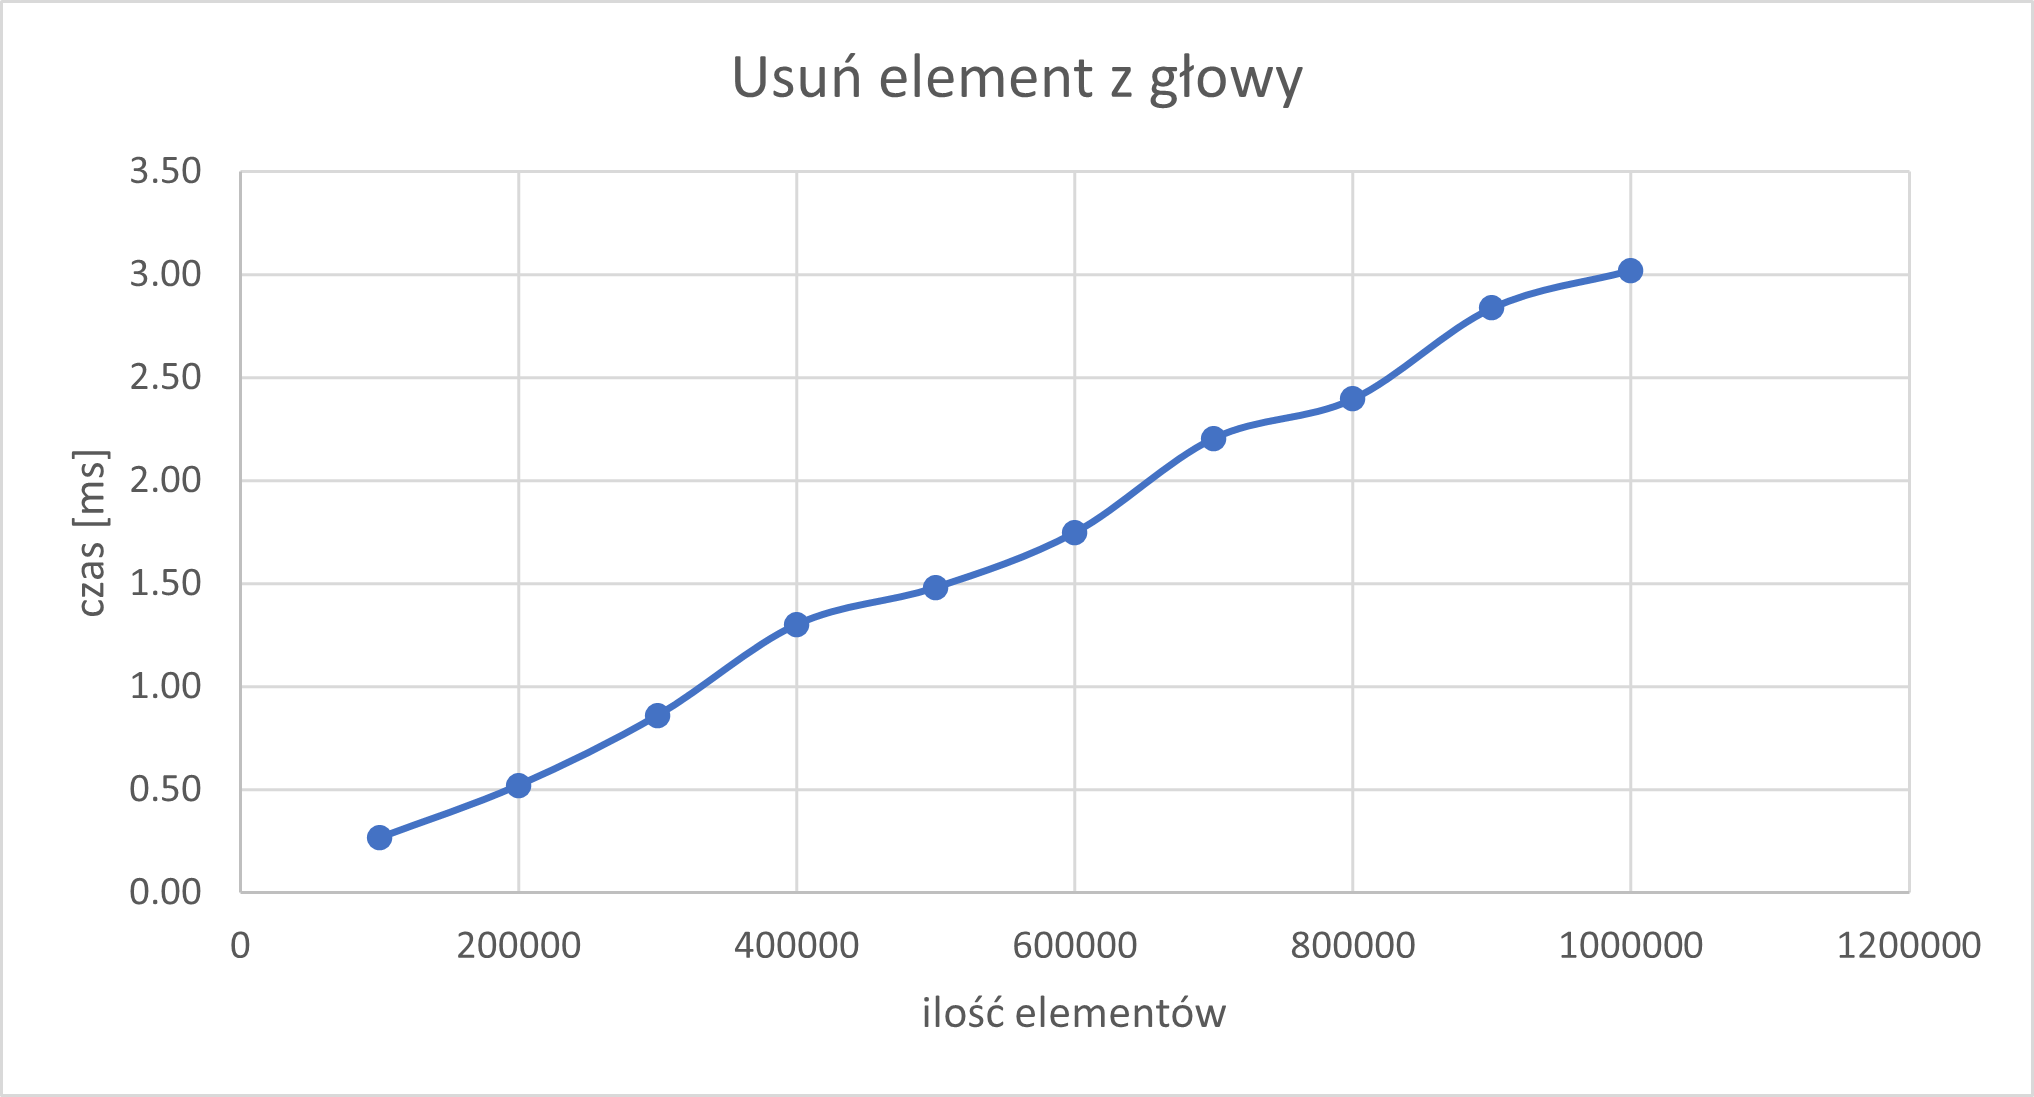
\includegraphics[scale = 0.85]{wykresy/heap/pop.png}
        \caption{Wykres czasu od ilości elementów dla Kopca - usuń z głowy (pop)}
    \end{figure}
    
    \begin{figure}[H]
        \centering
        \includegraphics[scale = 0.85]{wykresy/heap/find.png}
        \caption{Wykres czasu od ilości elementów dla Kopca - znajdź element}
    \end{figure}  



    \subsection{Wyniki testów dla drzewa czerwono-czarnego}
    \begin{table}[H]
        \centering
        \begin{tabular}{|c|ccc|}
            \hline
            \multirow{2}{*}{\textbf{Ilość   elementów}} & \multicolumn{3}{c|}{\textbf{Czas   potrzebny na wykonanie operacji {[}us{]}}} \\ \cline{2-4} 
             & \multicolumn{1}{c|}{\textbf{Dodaj element}} & \multicolumn{1}{c|}{\textbf{Usuń element}} & \textbf{Znajdź element} \\ \hline
            100000 & \multicolumn{1}{c|}{0.42} & \multicolumn{1}{c|}{1.69} & 0.27 \\ \hline
            200000 & \multicolumn{1}{c|}{0.53} & \multicolumn{1}{c|}{1.77} & 0.47 \\ \hline
            300000 & \multicolumn{1}{c|}{0.69} & \multicolumn{1}{c|}{1.99} & 0.60 \\ \hline
            400000 & \multicolumn{1}{c|}{0.78} & \multicolumn{1}{c|}{2.09} & 0.54 \\ \hline
            500000 & \multicolumn{1}{c|}{0.78} & \multicolumn{1}{c|}{2.04} & 0.64 \\ \hline
            600000 & \multicolumn{1}{c|}{1.08} & \multicolumn{1}{c|}{2.16} & 0.84 \\ \hline
            700000 & \multicolumn{1}{c|}{0.94} & \multicolumn{1}{c|}{2.41} & 0.67 \\ \hline
            800000 & \multicolumn{1}{c|}{0.88} & \multicolumn{1}{c|}{2.08} & 0.80 \\ \hline
            900000 & \multicolumn{1}{c|}{1.03} & \multicolumn{1}{c|}{2.22} & 0.76 \\ \hline
            1000000 & \multicolumn{1}{c|}{1.19} & \multicolumn{1}{c|}{2.44} & 0.81 \\ \hline
        \end{tabular}
        \caption{Pomiary drzewa czerwono-czarnego}
        % \label{tab:my-table}
    \end{table}

    
    \begin{figure}[H]
        \centering
        \includegraphics[scale = 0.85]{wykresy/rbt/add.png}
        \caption{Wykres czasu od ilości elementów dla Drzewa czerwono-czarnego - dodaj element}
    \end{figure}
    
    \begin{figure}[H]
        \centering
        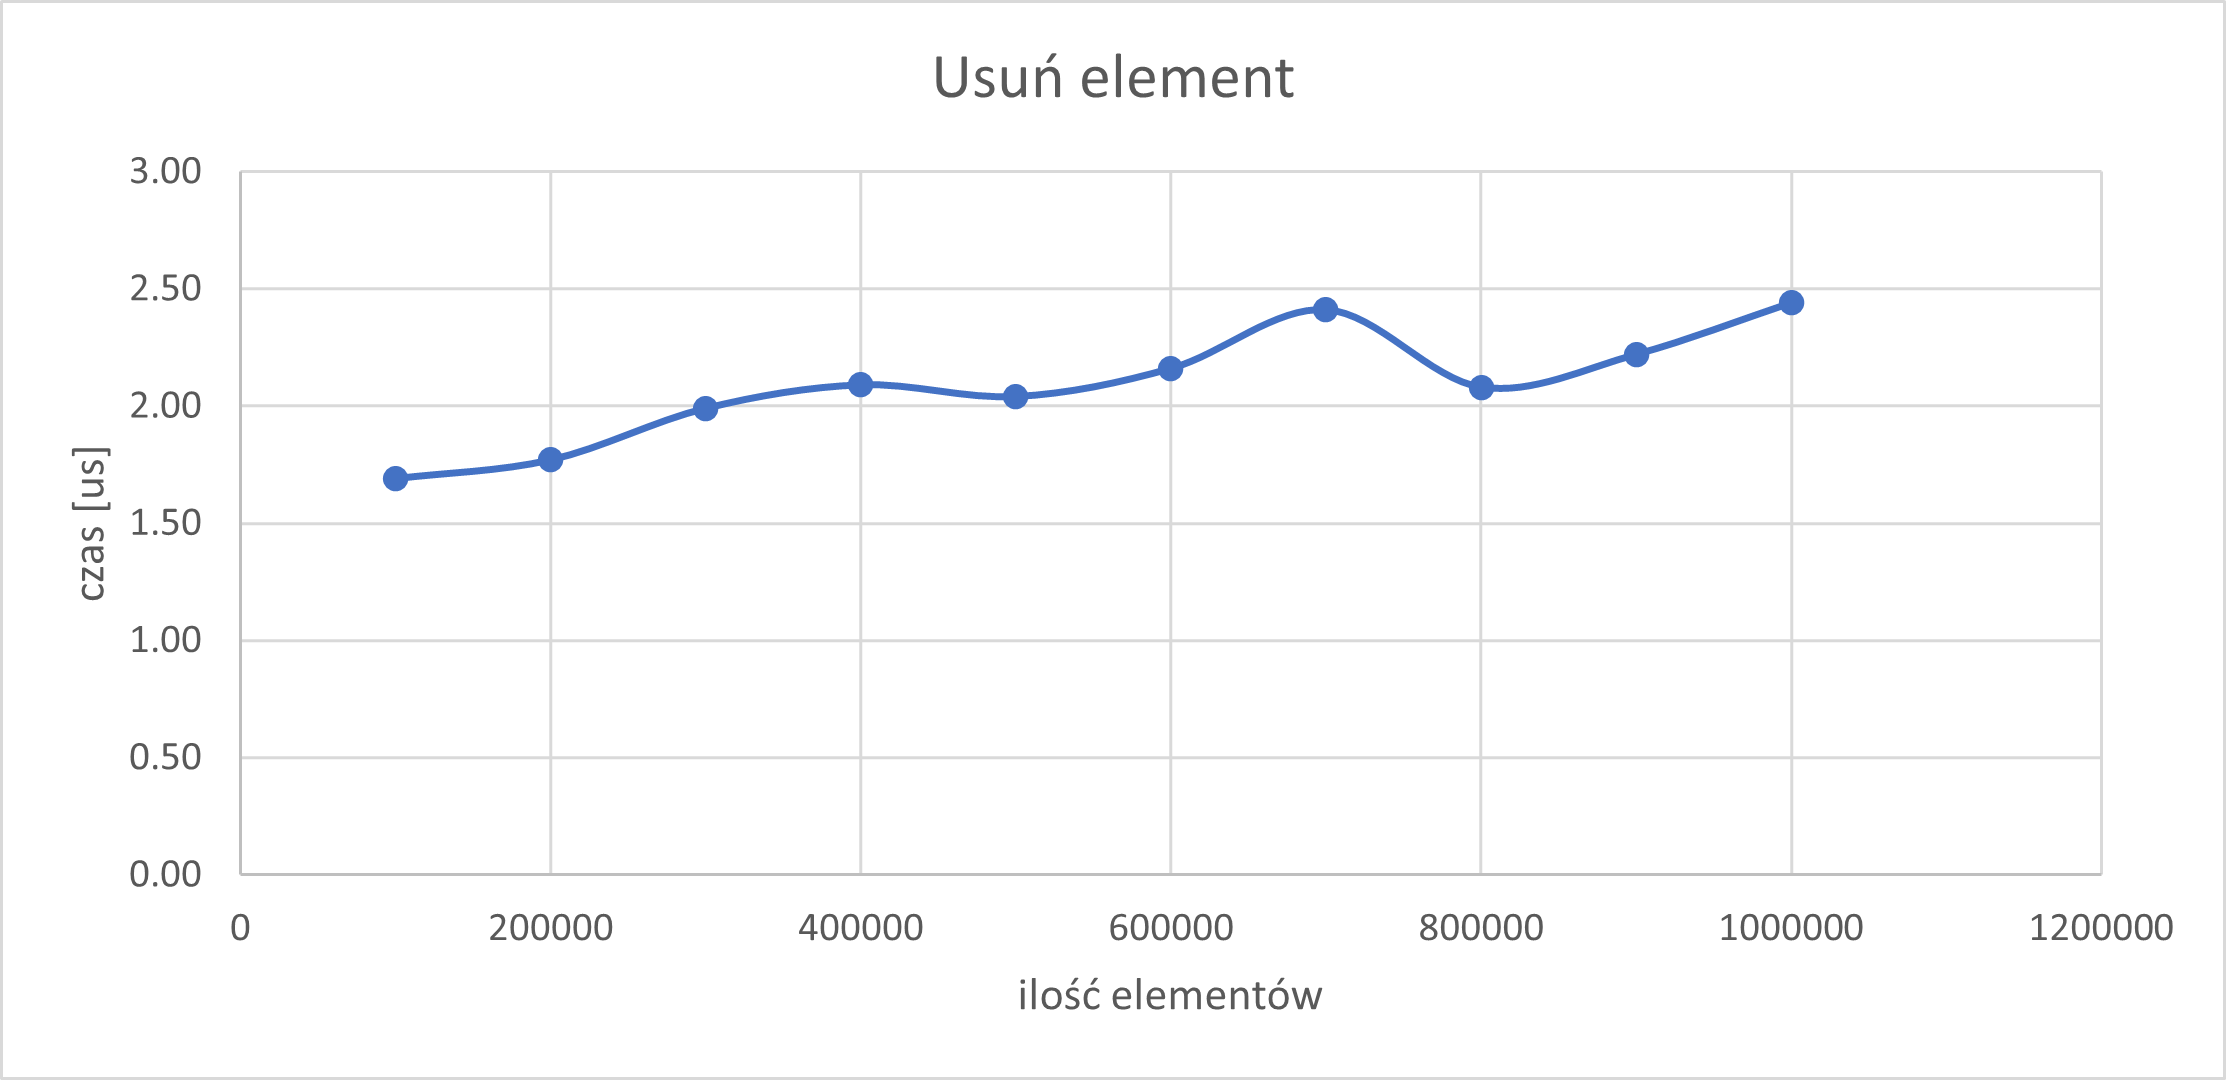
\includegraphics[scale = 0.85]{wykresy/rbt/remove.png}
        \caption{Wykres czasu od ilości elementów dla Drzewa czerwono-czarnego - usuń element}
    \end{figure}
    
    \begin{figure}[H]
        \centering
        \includegraphics[scale = 0.85]{wykresy/rbt/find.png}
        \caption{Wykres czasu od ilości elementów dla Drzewa czerwono-czarnego - znajdź element}
    \end{figure}  


\section{Wnioski}
    \subsection{Przykładowe wyliczenia}
        W tej sekcji porównane zostaną czasy otrzymane eksperymentalnie z tymi wynikającymi z teorii. Porównywane będą zależności
        czasu wykonania danych operacji dla rozmiarów:
        \begin{itemize}
            \item 400 tysięcy i 100 tysięcy (proporcja 4:1)
            \item 800 tysięcy i 100 tysięcy (proporcja 8:1)
            \item 800 tysięcy i 200 tysięcy (proporcja 4:1)
        \end{itemize}

        \subsubsection*{Tablica dynamiczna}
            \begin{table}[H]
                \centering
                \resizebox{\columnwidth}{!}{%
                \begin{tabular}{|ccccccc|}
                    \hline
                    \multicolumn{7}{|c|}{\textbf{Wybrane wyliczenia porównujące czasy operacji   tablicy dynamicznej z teorią}} \\ \hline
                    \multicolumn{1}{|c|}{\textbf{Rodzaj operacji}} & \multicolumn{1}{c|}{\textbf{\begin{tabular}[c]{@{}c@{}}Teoretyczna   \\ złożoność\end{tabular}}} & \multicolumn{1}{c|}{\textbf{Ilość elementów}} & \multicolumn{1}{c|}{\textbf{\begin{tabular}[c]{@{}c@{}}Czas otrzymany   \\ eksperymentalnie\end{tabular}}} & \multicolumn{1}{c|}{\textbf{\begin{tabular}[c]{@{}c@{}}Stosunek ilości  \\  elementów\end{tabular}}} & \multicolumn{1}{c|}{\textbf{\begin{tabular}[c]{@{}c@{}}Teoretyczny czas   \\ wykonania operacji\end{tabular}}} & \textbf{Różnica} \\ \hline
                    \rowcolor[HTML]{F4FFF4} 
                    \multicolumn{1}{|c|}{\cellcolor[HTML]{F4FFF4}} & \multicolumn{1}{c|}{\cellcolor[HTML]{F4FFF4}} & \multicolumn{1}{c|}{\cellcolor[HTML]{F4FFF4}100000} & \multicolumn{1}{c|}{\cellcolor[HTML]{F4FFF4}0.31} & \multicolumn{1}{c|}{\cellcolor[HTML]{F4FFF4}} & \multicolumn{1}{c|}{\cellcolor[HTML]{F4FFF4}X} & X \\ \cline{3-4} \cline{6-7} 
                    \rowcolor[HTML]{F4FFF4} 
                    \multicolumn{1}{|c|}{\cellcolor[HTML]{F4FFF4}} & \multicolumn{1}{c|}{\cellcolor[HTML]{F4FFF4}} & \multicolumn{1}{c|}{\cellcolor[HTML]{F4FFF4}400000} & \multicolumn{1}{c|}{\cellcolor[HTML]{F4FFF4}1.46} & \multicolumn{1}{c|}{\multirow{-2}{*}{\cellcolor[HTML]{F4FFF4}4}} & \multicolumn{1}{c|}{\cellcolor[HTML]{F4FFF4}1.25} & 15\% \\ \cline{3-7} 
                    \rowcolor[HTML]{F4FFF4} 
                    \multicolumn{1}{|c|}{\cellcolor[HTML]{F4FFF4}} & \multicolumn{1}{c|}{\cellcolor[HTML]{F4FFF4}} & \multicolumn{1}{c|}{\cellcolor[HTML]{F4FFF4}100000} & \multicolumn{1}{c|}{\cellcolor[HTML]{F4FFF4}0.31} & \multicolumn{1}{c|}{\cellcolor[HTML]{F4FFF4}} & \multicolumn{1}{c|}{\cellcolor[HTML]{F4FFF4}X} & X \\ \cline{3-4} \cline{6-7} 
                    \rowcolor[HTML]{F4FFF4} 
                    \multicolumn{1}{|c|}{\cellcolor[HTML]{F4FFF4}} & \multicolumn{1}{c|}{\cellcolor[HTML]{F4FFF4}} & \multicolumn{1}{c|}{\cellcolor[HTML]{F4FFF4}800000} & \multicolumn{1}{c|}{\cellcolor[HTML]{F4FFF4}2.83} & \multicolumn{1}{c|}{\multirow{-2}{*}{\cellcolor[HTML]{F4FFF4}8}} & \multicolumn{1}{c|}{\cellcolor[HTML]{F4FFF4}2.50} & 12\% \\ \cline{3-7} 
                    \rowcolor[HTML]{F4FFF4} 
                    \multicolumn{1}{|c|}{\cellcolor[HTML]{F4FFF4}} & \multicolumn{1}{c|}{\cellcolor[HTML]{F4FFF4}} & \multicolumn{1}{c|}{\cellcolor[HTML]{F4FFF4}200000} & \multicolumn{1}{c|}{\cellcolor[HTML]{F4FFF4}0.69} & \multicolumn{1}{c|}{\cellcolor[HTML]{F4FFF4}} & \multicolumn{1}{c|}{\cellcolor[HTML]{F4FFF4}X} & X \\ \cline{3-4} \cline{6-7} 
                    \rowcolor[HTML]{F4FFF4} 
                    \multicolumn{1}{|c|}{\multirow{-6}{*}{\cellcolor[HTML]{F4FFF4}Dodaj   na początek}} & \multicolumn{1}{c|}{\multirow{-6}{*}{\cellcolor[HTML]{F4FFF4}O(n)}} & \multicolumn{1}{c|}{\cellcolor[HTML]{F4FFF4}800000} & \multicolumn{1}{c|}{\cellcolor[HTML]{F4FFF4}2.83} & \multicolumn{1}{c|}{\multirow{-2}{*}{\cellcolor[HTML]{F4FFF4}4}} & \multicolumn{1}{c|}{\cellcolor[HTML]{F4FFF4}2.75} & 3\% \\ \hline
                    \multicolumn{1}{|c|}{} & \multicolumn{1}{c|}{} & \multicolumn{1}{c|}{100000} & \multicolumn{1}{c|}{0.27} & \multicolumn{1}{c|}{} & \multicolumn{1}{c|}{X} & X \\ \cline{3-4} \cline{6-7} 
                    \multicolumn{1}{|c|}{} & \multicolumn{1}{c|}{} & \multicolumn{1}{c|}{400000} & \multicolumn{1}{c|}{1.63} & \multicolumn{1}{c|}{\multirow{-2}{*}{4}} & \multicolumn{1}{c|}{1.09} & 33\% \\ \cline{3-7} 
                    \multicolumn{1}{|c|}{} & \multicolumn{1}{c|}{} & \multicolumn{1}{c|}{100000} & \multicolumn{1}{c|}{0.27} & \multicolumn{1}{c|}{} & \multicolumn{1}{c|}{X} & X \\ \cline{3-4} \cline{6-7} 
                    \multicolumn{1}{|c|}{} & \multicolumn{1}{c|}{} & \multicolumn{1}{c|}{800000} & \multicolumn{1}{c|}{2.98} & \multicolumn{1}{c|}{\multirow{-2}{*}{8}} & \multicolumn{1}{c|}{2.19} & 26\% \\ \cline{3-7} 
                    \multicolumn{1}{|c|}{} & \multicolumn{1}{c|}{} & \multicolumn{1}{c|}{200000} & \multicolumn{1}{c|}{0.60} & \multicolumn{1}{c|}{} & \multicolumn{1}{c|}{X} & X \\ \cline{3-4} \cline{6-7} 
                    \multicolumn{1}{|c|}{\multirow{-6}{*}{Dodaj   na koniec}} & \multicolumn{1}{c|}{\multirow{-6}{*}{O(n)}} & \multicolumn{1}{c|}{800000} & \multicolumn{1}{c|}{2.98} & \multicolumn{1}{c|}{\multirow{-2}{*}{4}} & \multicolumn{1}{c|}{2.40} & 19\% \\ \hline
                    \rowcolor[HTML]{F4FFF4} 
                    \multicolumn{1}{|c|}{\cellcolor[HTML]{F4FFF4}} & \multicolumn{1}{c|}{\cellcolor[HTML]{F4FFF4}} & \multicolumn{1}{c|}{\cellcolor[HTML]{F4FFF4}100000} & \multicolumn{1}{c|}{\cellcolor[HTML]{F4FFF4}0.28} & \multicolumn{1}{c|}{\cellcolor[HTML]{F4FFF4}} & \multicolumn{1}{c|}{\cellcolor[HTML]{F4FFF4}X} & X \\ \cline{3-4} \cline{6-7} 
                    \rowcolor[HTML]{F4FFF4} 
                    \multicolumn{1}{|c|}{\cellcolor[HTML]{F4FFF4}} & \multicolumn{1}{c|}{\cellcolor[HTML]{F4FFF4}} & \multicolumn{1}{c|}{\cellcolor[HTML]{F4FFF4}400000} & \multicolumn{1}{c|}{\cellcolor[HTML]{F4FFF4}1.46} & \multicolumn{1}{c|}{\multirow{-2}{*}{\cellcolor[HTML]{F4FFF4}4}} & \multicolumn{1}{c|}{\cellcolor[HTML]{F4FFF4}1.12} & 23\% \\ \cline{3-7} 
                    \rowcolor[HTML]{F4FFF4} 
                    \multicolumn{1}{|c|}{\cellcolor[HTML]{F4FFF4}} & \multicolumn{1}{c|}{\cellcolor[HTML]{F4FFF4}} & \multicolumn{1}{c|}{\cellcolor[HTML]{F4FFF4}100000} & \multicolumn{1}{c|}{\cellcolor[HTML]{F4FFF4}0.28} & \multicolumn{1}{c|}{\cellcolor[HTML]{F4FFF4}} & \multicolumn{1}{c|}{\cellcolor[HTML]{F4FFF4}X} & X \\ \cline{3-4} \cline{6-7} 
                    \rowcolor[HTML]{F4FFF4} 
                    \multicolumn{1}{|c|}{\cellcolor[HTML]{F4FFF4}} & \multicolumn{1}{c|}{\cellcolor[HTML]{F4FFF4}} & \multicolumn{1}{c|}{\cellcolor[HTML]{F4FFF4}800000} & \multicolumn{1}{c|}{\cellcolor[HTML]{F4FFF4}3.05} & \multicolumn{1}{c|}{\multirow{-2}{*}{\cellcolor[HTML]{F4FFF4}8}} & \multicolumn{1}{c|}{\cellcolor[HTML]{F4FFF4}2.24} & 26\% \\ \cline{3-7} 
                    \rowcolor[HTML]{F4FFF4} 
                    \multicolumn{1}{|c|}{\cellcolor[HTML]{F4FFF4}} & \multicolumn{1}{c|}{\cellcolor[HTML]{F4FFF4}} & \multicolumn{1}{c|}{\cellcolor[HTML]{F4FFF4}200000} & \multicolumn{1}{c|}{\cellcolor[HTML]{F4FFF4}0.69} & \multicolumn{1}{c|}{\cellcolor[HTML]{F4FFF4}} & \multicolumn{1}{c|}{\cellcolor[HTML]{F4FFF4}X} & X \\ \cline{3-4} \cline{6-7} 
                    \rowcolor[HTML]{F4FFF4} 
                    \multicolumn{1}{|c|}{\multirow{-6}{*}{\cellcolor[HTML]{F4FFF4}\begin{tabular}[c]{@{}c@{}}Dodaj w \\ wybrane miejsce\end{tabular}}} & \multicolumn{1}{c|}{\multirow{-6}{*}{\cellcolor[HTML]{F4FFF4}O(n)}} & \multicolumn{1}{c|}{\cellcolor[HTML]{F4FFF4}800000} & \multicolumn{1}{c|}{\cellcolor[HTML]{F4FFF4}3.05} & \multicolumn{1}{c|}{\multirow{-2}{*}{\cellcolor[HTML]{F4FFF4}4}} & \multicolumn{1}{c|}{\cellcolor[HTML]{F4FFF4}2.77} & 9\% \\ \hline
                    \multicolumn{1}{|c|}{} & \multicolumn{1}{c|}{} & \multicolumn{1}{c|}{100000} & \multicolumn{1}{c|}{0.25} & \multicolumn{1}{c|}{} & \multicolumn{1}{c|}{X} & X \\ \cline{3-4} \cline{6-7} 
                    \multicolumn{1}{|c|}{} & \multicolumn{1}{c|}{} & \multicolumn{1}{c|}{400000} & \multicolumn{1}{c|}{1.57} & \multicolumn{1}{c|}{\multirow{-2}{*}{4}} & \multicolumn{1}{c|}{0.99} & 37\% \\ \cline{3-7} 
                    \multicolumn{1}{|c|}{} & \multicolumn{1}{c|}{} & \multicolumn{1}{c|}{100000} & \multicolumn{1}{c|}{0.25} & \multicolumn{1}{c|}{} & \multicolumn{1}{c|}{X} & X \\ \cline{3-4} \cline{6-7} 
                    \multicolumn{1}{|c|}{} & \multicolumn{1}{c|}{} & \multicolumn{1}{c|}{800000} & \multicolumn{1}{c|}{2.56} & \multicolumn{1}{c|}{\multirow{-2}{*}{8}} & \multicolumn{1}{c|}{1.98} & 23\% \\ \cline{3-7} 
                    \multicolumn{1}{|c|}{} & \multicolumn{1}{c|}{} & \multicolumn{1}{c|}{200000} & \multicolumn{1}{c|}{0.66} & \multicolumn{1}{c|}{} & \multicolumn{1}{c|}{X} & X \\ \cline{3-4} \cline{6-7} 
                    \multicolumn{1}{|c|}{\multirow{-6}{*}{Usuń z początku}} & \multicolumn{1}{c|}{\multirow{-6}{*}{O(n)}} & \multicolumn{1}{c|}{800000} & \multicolumn{1}{c|}{2.56} & \multicolumn{1}{c|}{\multirow{-2}{*}{4}} & \multicolumn{1}{c|}{2.64} & 3\% \\ \hline
                    \rowcolor[HTML]{F4FFF4} 
                    \multicolumn{1}{|c|}{\cellcolor[HTML]{F4FFF4}} & \multicolumn{1}{c|}{\cellcolor[HTML]{F4FFF4}} & \multicolumn{1}{c|}{\cellcolor[HTML]{F4FFF4}100000} & \multicolumn{1}{c|}{\cellcolor[HTML]{F4FFF4}0.26} & \multicolumn{1}{c|}{\cellcolor[HTML]{F4FFF4}} & \multicolumn{1}{c|}{\cellcolor[HTML]{F4FFF4}X} & X \\ \cline{3-4} \cline{6-7} 
                    \rowcolor[HTML]{F4FFF4} 
                    \multicolumn{1}{|c|}{\cellcolor[HTML]{F4FFF4}} & \multicolumn{1}{c|}{\cellcolor[HTML]{F4FFF4}} & \multicolumn{1}{c|}{\cellcolor[HTML]{F4FFF4}400000} & \multicolumn{1}{c|}{\cellcolor[HTML]{F4FFF4}1.46} & \multicolumn{1}{c|}{\multirow{-2}{*}{\cellcolor[HTML]{F4FFF4}4}} & \multicolumn{1}{c|}{\cellcolor[HTML]{F4FFF4}1.06} & 27\% \\ \cline{3-7} 
                    \rowcolor[HTML]{F4FFF4} 
                    \multicolumn{1}{|c|}{\cellcolor[HTML]{F4FFF4}} & \multicolumn{1}{c|}{\cellcolor[HTML]{F4FFF4}} & \multicolumn{1}{c|}{\cellcolor[HTML]{F4FFF4}100000} & \multicolumn{1}{c|}{\cellcolor[HTML]{F4FFF4}0.26} & \multicolumn{1}{c|}{\cellcolor[HTML]{F4FFF4}} & \multicolumn{1}{c|}{\cellcolor[HTML]{F4FFF4}X} & X \\ \cline{3-4} \cline{6-7} 
                    \rowcolor[HTML]{F4FFF4} 
                    \multicolumn{1}{|c|}{\cellcolor[HTML]{F4FFF4}} & \multicolumn{1}{c|}{\cellcolor[HTML]{F4FFF4}} & \multicolumn{1}{c|}{\cellcolor[HTML]{F4FFF4}800000} & \multicolumn{1}{c|}{\cellcolor[HTML]{F4FFF4}2.66} & \multicolumn{1}{c|}{\multirow{-2}{*}{\cellcolor[HTML]{F4FFF4}8}} & \multicolumn{1}{c|}{\cellcolor[HTML]{F4FFF4}2.12} & 20\% \\ \cline{3-7} 
                    \rowcolor[HTML]{F4FFF4} 
                    \multicolumn{1}{|c|}{\cellcolor[HTML]{F4FFF4}} & \multicolumn{1}{c|}{\cellcolor[HTML]{F4FFF4}} & \multicolumn{1}{c|}{\cellcolor[HTML]{F4FFF4}200000} & \multicolumn{1}{c|}{\cellcolor[HTML]{F4FFF4}0.62} & \multicolumn{1}{c|}{\cellcolor[HTML]{F4FFF4}} & \multicolumn{1}{c|}{\cellcolor[HTML]{F4FFF4}X} & X \\ \cline{3-4} \cline{6-7} 
                    \rowcolor[HTML]{F4FFF4} 
                    \multicolumn{1}{|c|}{\multirow{-6}{*}{\cellcolor[HTML]{F4FFF4}Usuń z końca}} & \multicolumn{1}{c|}{\multirow{-6}{*}{\cellcolor[HTML]{F4FFF4}O(n)}} & \multicolumn{1}{c|}{\cellcolor[HTML]{F4FFF4}800000} & \multicolumn{1}{c|}{\cellcolor[HTML]{F4FFF4}2.66} & \multicolumn{1}{c|}{\multirow{-2}{*}{\cellcolor[HTML]{F4FFF4}4}} & \multicolumn{1}{c|}{\cellcolor[HTML]{F4FFF4}2.46} & 7\% \\ \hline
                    \multicolumn{1}{|c|}{} & \multicolumn{1}{c|}{} & \multicolumn{1}{c|}{100000} & \multicolumn{1}{c|}{0.25} & \multicolumn{1}{c|}{} & \multicolumn{1}{c|}{X} & X \\ \cline{3-4} \cline{6-7} 
                    \multicolumn{1}{|c|}{} & \multicolumn{1}{c|}{} & \multicolumn{1}{c|}{400000} & \multicolumn{1}{c|}{1.30} & \multicolumn{1}{c|}{\multirow{-2}{*}{4}} & \multicolumn{1}{c|}{1.01} & 22\% \\ \cline{3-7} 
                    \multicolumn{1}{|c|}{} & \multicolumn{1}{c|}{} & \multicolumn{1}{c|}{100000} & \multicolumn{1}{c|}{0.25} & \multicolumn{1}{c|}{} & \multicolumn{1}{c|}{X} & X \\ \cline{3-4} \cline{6-7} 
                    \multicolumn{1}{|c|}{} & \multicolumn{1}{c|}{} & \multicolumn{1}{c|}{800000} & \multicolumn{1}{c|}{2.86} & \multicolumn{1}{c|}{\multirow{-2}{*}{8}} & \multicolumn{1}{c|}{2.03} & 29\% \\ \cline{3-7} 
                    \multicolumn{1}{|c|}{} & \multicolumn{1}{c|}{} & \multicolumn{1}{c|}{200000} & \multicolumn{1}{c|}{0.62} & \multicolumn{1}{c|}{} & \multicolumn{1}{c|}{X} & X \\ \cline{3-4} \cline{6-7} 
                    \multicolumn{1}{|c|}{\multirow{-6}{*}{\begin{tabular}[c]{@{}c@{}}Usuń z \\ wybranego miejsca\end{tabular}}} & \multicolumn{1}{c|}{\multirow{-6}{*}{O(n)}} & \multicolumn{1}{c|}{800000} & \multicolumn{1}{c|}{2.86} & \multicolumn{1}{c|}{\multirow{-2}{*}{4}} & \multicolumn{1}{c|}{2.48} & 13\% \\ \hline
                    \rowcolor[HTML]{F4FFF4} 
                    \multicolumn{1}{|c|}{\cellcolor[HTML]{F4FFF4}} & \multicolumn{1}{c|}{\cellcolor[HTML]{F4FFF4}} & \multicolumn{1}{c|}{\cellcolor[HTML]{F4FFF4}100000} & \multicolumn{1}{c|}{\cellcolor[HTML]{F4FFF4}0.20} & \multicolumn{1}{c|}{\cellcolor[HTML]{F4FFF4}} & \multicolumn{1}{c|}{\cellcolor[HTML]{F4FFF4}X} & X \\ \cline{3-4} \cline{6-7} 
                    \rowcolor[HTML]{F4FFF4} 
                    \multicolumn{1}{|c|}{\cellcolor[HTML]{F4FFF4}} & \multicolumn{1}{c|}{\cellcolor[HTML]{F4FFF4}} & \multicolumn{1}{c|}{\cellcolor[HTML]{F4FFF4}400000} & \multicolumn{1}{c|}{\cellcolor[HTML]{F4FFF4}0.67} & \multicolumn{1}{c|}{\multirow{-2}{*}{\cellcolor[HTML]{F4FFF4}4}} & \multicolumn{1}{c|}{\cellcolor[HTML]{F4FFF4}0.82} & 18\% \\ \cline{3-7} 
                    \rowcolor[HTML]{F4FFF4} 
                    \multicolumn{1}{|c|}{\cellcolor[HTML]{F4FFF4}} & \multicolumn{1}{c|}{\cellcolor[HTML]{F4FFF4}} & \multicolumn{1}{c|}{\cellcolor[HTML]{F4FFF4}100000} & \multicolumn{1}{c|}{\cellcolor[HTML]{F4FFF4}0.20} & \multicolumn{1}{c|}{\cellcolor[HTML]{F4FFF4}} & \multicolumn{1}{c|}{\cellcolor[HTML]{F4FFF4}X} & X \\ \cline{3-4} \cline{6-7} 
                    \rowcolor[HTML]{F4FFF4} 
                    \multicolumn{1}{|c|}{\cellcolor[HTML]{F4FFF4}} & \multicolumn{1}{c|}{\cellcolor[HTML]{F4FFF4}} & \multicolumn{1}{c|}{\cellcolor[HTML]{F4FFF4}800000} & \multicolumn{1}{c|}{\cellcolor[HTML]{F4FFF4}1.53} & \multicolumn{1}{c|}{\multirow{-2}{*}{\cellcolor[HTML]{F4FFF4}8}} & \multicolumn{1}{c|}{\cellcolor[HTML]{F4FFF4}1.64} & 7\% \\ \cline{3-7} 
                    \rowcolor[HTML]{F4FFF4} 
                    \multicolumn{1}{|c|}{\cellcolor[HTML]{F4FFF4}} & \multicolumn{1}{c|}{\cellcolor[HTML]{F4FFF4}} & \multicolumn{1}{c|}{\cellcolor[HTML]{F4FFF4}200000} & \multicolumn{1}{c|}{\cellcolor[HTML]{F4FFF4}0.30} & \multicolumn{1}{c|}{\cellcolor[HTML]{F4FFF4}} & \multicolumn{1}{c|}{\cellcolor[HTML]{F4FFF4}X} & X \\ \cline{3-4} \cline{6-7} 
                    \rowcolor[HTML]{F4FFF4} 
                    \multicolumn{1}{|c|}{\multirow{-6}{*}{\cellcolor[HTML]{F4FFF4}Znajdź element}} & \multicolumn{1}{c|}{\multirow{-6}{*}{\cellcolor[HTML]{F4FFF4}O(n)}} & \multicolumn{1}{c|}{\cellcolor[HTML]{F4FFF4}800000} & \multicolumn{1}{c|}{\cellcolor[HTML]{F4FFF4}1.53} & \multicolumn{1}{c|}{\multirow{-2}{*}{\cellcolor[HTML]{F4FFF4}4}} & \multicolumn{1}{c|}{\cellcolor[HTML]{F4FFF4}1.21} & 21\% \\ \hline
                    \end{tabular}%
                    }
                \caption{Porównanie otrzymanych czasów dla tablicy dynamicznej z teorią}
                % \label{tab:my-table}
            \end{table}


        \subsubsection*{Lista dwukierunkowa}
        \begin{table}[H]
            \centering
            \resizebox{\columnwidth}{!}{%
            \begin{tabular}{|ccccccc|}
                \hline
                \multicolumn{7}{|c|}{\textbf{Wybrane wyliczenia porównujące czasy operacji   listy dwukierunkowej z teorią}} \\ \hline
                \multicolumn{1}{|c|}{\textbf{Rodzaj operacji}} & \multicolumn{1}{c|}{\textbf{\begin{tabular}[c]{@{}c@{}}Teoretyczna \\   złożoność\end{tabular}}} & \multicolumn{1}{c|}{\textbf{Ilość elementów}} & \multicolumn{1}{c|}{\textbf{\begin{tabular}[c]{@{}c@{}}Czas otrzymany  \\  eksperymentalnie\end{tabular}}} & \multicolumn{1}{c|}{\textbf{\begin{tabular}[c]{@{}c@{}}Stosunek ilości  \\  elementów\end{tabular}}} & \multicolumn{1}{c|}{\textbf{\begin{tabular}[c]{@{}c@{}}Teoretyczny czas  \\  wykonania operacji\end{tabular}}} & \textbf{Różnica} \\ \hline
                \rowcolor[HTML]{F4FFF4} 
                \multicolumn{1}{|c|}{\cellcolor[HTML]{F4FFF4}} & \multicolumn{1}{c|}{\cellcolor[HTML]{F4FFF4}} & \multicolumn{1}{c|}{\cellcolor[HTML]{F4FFF4}100000} & \multicolumn{1}{c|}{\cellcolor[HTML]{F4FFF4}0.11} & \multicolumn{1}{c|}{\cellcolor[HTML]{F4FFF4}} & \multicolumn{1}{c|}{\cellcolor[HTML]{F4FFF4}X} & X \\ \cline{3-4} \cline{6-7} 
                \rowcolor[HTML]{F4FFF4} 
                \multicolumn{1}{|c|}{\cellcolor[HTML]{F4FFF4}} & \multicolumn{1}{c|}{\cellcolor[HTML]{F4FFF4}} & \multicolumn{1}{c|}{\cellcolor[HTML]{F4FFF4}400000} & \multicolumn{1}{c|}{\cellcolor[HTML]{F4FFF4}0.12} & \multicolumn{1}{c|}{\multirow{-2}{*}{\cellcolor[HTML]{F4FFF4}4}} & \multicolumn{1}{c|}{\cellcolor[HTML]{F4FFF4}0.11} & 7\% \\ \cline{3-7} 
                \rowcolor[HTML]{F4FFF4} 
                \multicolumn{1}{|c|}{\cellcolor[HTML]{F4FFF4}} & \multicolumn{1}{c|}{\cellcolor[HTML]{F4FFF4}} & \multicolumn{1}{c|}{\cellcolor[HTML]{F4FFF4}100000} & \multicolumn{1}{c|}{\cellcolor[HTML]{F4FFF4}0.11} & \multicolumn{1}{c|}{\cellcolor[HTML]{F4FFF4}} & \multicolumn{1}{c|}{\cellcolor[HTML]{F4FFF4}X} & X \\ \cline{3-4} \cline{6-7} 
                \rowcolor[HTML]{F4FFF4} 
                \multicolumn{1}{|c|}{\cellcolor[HTML]{F4FFF4}} & \multicolumn{1}{c|}{\cellcolor[HTML]{F4FFF4}} & \multicolumn{1}{c|}{\cellcolor[HTML]{F4FFF4}800000} & \multicolumn{1}{c|}{\cellcolor[HTML]{F4FFF4}0.12} & \multicolumn{1}{c|}{\multirow{-2}{*}{\cellcolor[HTML]{F4FFF4}8}} & \multicolumn{1}{c|}{\cellcolor[HTML]{F4FFF4}0.11} & 7\% \\ \cline{3-7} 
                \rowcolor[HTML]{F4FFF4} 
                \multicolumn{1}{|c|}{\cellcolor[HTML]{F4FFF4}} & \multicolumn{1}{c|}{\cellcolor[HTML]{F4FFF4}} & \multicolumn{1}{c|}{\cellcolor[HTML]{F4FFF4}200000} & \multicolumn{1}{c|}{\cellcolor[HTML]{F4FFF4}0.14} & \multicolumn{1}{c|}{\cellcolor[HTML]{F4FFF4}} & \multicolumn{1}{c|}{\cellcolor[HTML]{F4FFF4}X} & X \\ \cline{3-4} \cline{6-7} 
                \rowcolor[HTML]{F4FFF4} 
                \multicolumn{1}{|c|}{\multirow{-6}{*}{\cellcolor[HTML]{F4FFF4}Dodaj na początek}} & \multicolumn{1}{c|}{\multirow{-6}{*}{\cellcolor[HTML]{F4FFF4}O(1)}} & \multicolumn{1}{c|}{\cellcolor[HTML]{F4FFF4}800000} & \multicolumn{1}{c|}{\cellcolor[HTML]{F4FFF4}0.12} & \multicolumn{1}{c|}{\multirow{-2}{*}{\cellcolor[HTML]{F4FFF4}4}} & \multicolumn{1}{c|}{\cellcolor[HTML]{F4FFF4}0.14} & 19\% \\ \hline
                \multicolumn{1}{|c|}{} & \multicolumn{1}{c|}{} & \multicolumn{1}{c|}{100000} & \multicolumn{1}{c|}{0.08} & \multicolumn{1}{c|}{} & \multicolumn{1}{c|}{X} & X \\ \cline{3-4} \cline{6-7} 
                \multicolumn{1}{|c|}{} & \multicolumn{1}{c|}{} & \multicolumn{1}{c|}{400000} & \multicolumn{1}{c|}{0.13} & \multicolumn{1}{c|}{\multirow{-2}{*}{4}} & \multicolumn{1}{c|}{0.08} & 43\% \\ \cline{3-7} 
                \multicolumn{1}{|c|}{} & \multicolumn{1}{c|}{} & \multicolumn{1}{c|}{100000} & \multicolumn{1}{c|}{0.08} & \multicolumn{1}{c|}{} & \multicolumn{1}{c|}{X} & X \\ \cline{3-4} \cline{6-7} 
                \multicolumn{1}{|c|}{} & \multicolumn{1}{c|}{} & \multicolumn{1}{c|}{800000} & \multicolumn{1}{c|}{0.09} & \multicolumn{1}{c|}{\multirow{-2}{*}{8}} & \multicolumn{1}{c|}{0.08} & 16\% \\ \cline{3-7} 
                \multicolumn{1}{|c|}{} & \multicolumn{1}{c|}{} & \multicolumn{1}{c|}{200000} & \multicolumn{1}{c|}{0.10} & \multicolumn{1}{c|}{} & \multicolumn{1}{c|}{X} & X \\ \cline{3-4} \cline{6-7} 
                \multicolumn{1}{|c|}{\multirow{-6}{*}{Dodaj na koniec}} & \multicolumn{1}{c|}{\multirow{-6}{*}{O(1)}} & \multicolumn{1}{c|}{800000} & \multicolumn{1}{c|}{0.09} & \multicolumn{1}{c|}{\multirow{-2}{*}{4}} & \multicolumn{1}{c|}{0.10} & 7\% \\ \hline
                \rowcolor[HTML]{F4FFF4} 
                \multicolumn{1}{|c|}{\cellcolor[HTML]{F4FFF4}} & \multicolumn{1}{c|}{\cellcolor[HTML]{F4FFF4}} & \multicolumn{1}{c|}{\cellcolor[HTML]{F4FFF4}100000} & \multicolumn{1}{c|}{\cellcolor[HTML]{F4FFF4}0.72} & \multicolumn{1}{c|}{\cellcolor[HTML]{F4FFF4}} & \multicolumn{1}{c|}{\cellcolor[HTML]{F4FFF4}X} & X \\ \cline{3-4} \cline{6-7} 
                \rowcolor[HTML]{F4FFF4} 
                \multicolumn{1}{|c|}{\cellcolor[HTML]{F4FFF4}} & \multicolumn{1}{c|}{\cellcolor[HTML]{F4FFF4}} & \multicolumn{1}{c|}{\cellcolor[HTML]{F4FFF4}400000} & \multicolumn{1}{c|}{\cellcolor[HTML]{F4FFF4}0.89} & \multicolumn{1}{c|}{\multirow{-2}{*}{\cellcolor[HTML]{F4FFF4}4}} & \multicolumn{1}{c|}{\cellcolor[HTML]{F4FFF4}0.72} & 19\% \\ \cline{3-7} 
                \rowcolor[HTML]{F4FFF4} 
                \multicolumn{1}{|c|}{\cellcolor[HTML]{F4FFF4}} & \multicolumn{1}{c|}{\cellcolor[HTML]{F4FFF4}} & \multicolumn{1}{c|}{\cellcolor[HTML]{F4FFF4}100000} & \multicolumn{1}{c|}{\cellcolor[HTML]{F4FFF4}0.72} & \multicolumn{1}{c|}{\cellcolor[HTML]{F4FFF4}} & \multicolumn{1}{c|}{\cellcolor[HTML]{F4FFF4}X} & X \\ \cline{3-4} \cline{6-7} 
                \rowcolor[HTML]{F4FFF4} 
                \multicolumn{1}{|c|}{\cellcolor[HTML]{F4FFF4}} & \multicolumn{1}{c|}{\cellcolor[HTML]{F4FFF4}} & \multicolumn{1}{c|}{\cellcolor[HTML]{F4FFF4}800000} & \multicolumn{1}{c|}{\cellcolor[HTML]{F4FFF4}0.66} & \multicolumn{1}{c|}{\multirow{-2}{*}{\cellcolor[HTML]{F4FFF4}8}} & \multicolumn{1}{c|}{\cellcolor[HTML]{F4FFF4}0.72} & 8\% \\ \cline{3-7} 
                \rowcolor[HTML]{F4FFF4} 
                \multicolumn{1}{|c|}{\cellcolor[HTML]{F4FFF4}} & \multicolumn{1}{c|}{\cellcolor[HTML]{F4FFF4}} & \multicolumn{1}{c|}{\cellcolor[HTML]{F4FFF4}200000} & \multicolumn{1}{c|}{\cellcolor[HTML]{F4FFF4}0.74} & \multicolumn{1}{c|}{\cellcolor[HTML]{F4FFF4}} & \multicolumn{1}{c|}{\cellcolor[HTML]{F4FFF4}X} & X \\ \cline{3-4} \cline{6-7} 
                \rowcolor[HTML]{F4FFF4} 
                \multicolumn{1}{|c|}{\multirow{-6}{*}{\cellcolor[HTML]{F4FFF4}Usuń z początku}} & \multicolumn{1}{c|}{\multirow{-6}{*}{\cellcolor[HTML]{F4FFF4}O(1)}} & \multicolumn{1}{c|}{\cellcolor[HTML]{F4FFF4}800000} & \multicolumn{1}{c|}{\cellcolor[HTML]{F4FFF4}0.66} & \multicolumn{1}{c|}{\multirow{-2}{*}{\cellcolor[HTML]{F4FFF4}4}} & \multicolumn{1}{c|}{\cellcolor[HTML]{F4FFF4}0.74} & 11\% \\ \hline
                \multicolumn{1}{|c|}{} & \multicolumn{1}{c|}{} & \multicolumn{1}{c|}{100000} & \multicolumn{1}{c|}{0.52} & \multicolumn{1}{c|}{} & \multicolumn{1}{c|}{X} & X \\ \cline{3-4} \cline{6-7} 
                \multicolumn{1}{|c|}{} & \multicolumn{1}{c|}{} & \multicolumn{1}{c|}{400000} & \multicolumn{1}{c|}{0.50} & \multicolumn{1}{c|}{\multirow{-2}{*}{4}} & \multicolumn{1}{c|}{0.52} & 3\% \\ \cline{3-7} 
                \multicolumn{1}{|c|}{} & \multicolumn{1}{c|}{} & \multicolumn{1}{c|}{100000} & \multicolumn{1}{c|}{0.52} & \multicolumn{1}{c|}{} & \multicolumn{1}{c|}{X} & X \\ \cline{3-4} \cline{6-7} 
                \multicolumn{1}{|c|}{} & \multicolumn{1}{c|}{} & \multicolumn{1}{c|}{800000} & \multicolumn{1}{c|}{0.48} & \multicolumn{1}{c|}{\multirow{-2}{*}{8}} & \multicolumn{1}{c|}{0.52} & 8\% \\ \cline{3-7} 
                \multicolumn{1}{|c|}{} & \multicolumn{1}{c|}{} & \multicolumn{1}{c|}{200000} & \multicolumn{1}{c|}{0.56} & \multicolumn{1}{c|}{} & \multicolumn{1}{c|}{X} & X \\ \cline{3-4} \cline{6-7} 
                \multicolumn{1}{|c|}{\multirow{-6}{*}{Usuń z końca}} & \multicolumn{1}{c|}{\multirow{-6}{*}{O(1)}} & \multicolumn{1}{c|}{800000} & \multicolumn{1}{c|}{0.48} & \multicolumn{1}{c|}{\multirow{-2}{*}{4}} & \multicolumn{1}{c|}{0.56} & 14\% \\ \hline
                \rowcolor[HTML]{F4FFF4} 
                \multicolumn{1}{|c|}{\cellcolor[HTML]{F4FFF4}} & \multicolumn{1}{c|}{\cellcolor[HTML]{F4FFF4}} & \multicolumn{1}{c|}{\cellcolor[HTML]{F4FFF4}100000} & \multicolumn{1}{c|}{\cellcolor[HTML]{F4FFF4}0.23} & \multicolumn{1}{c|}{\cellcolor[HTML]{F4FFF4}} & \multicolumn{1}{c|}{\cellcolor[HTML]{F4FFF4}X} & X \\ \cline{3-4} \cline{6-7} 
                \rowcolor[HTML]{F4FFF4} 
                \multicolumn{1}{|c|}{\cellcolor[HTML]{F4FFF4}} & \multicolumn{1}{c|}{\cellcolor[HTML]{F4FFF4}} & \multicolumn{1}{c|}{\cellcolor[HTML]{F4FFF4}400000} & \multicolumn{1}{c|}{\cellcolor[HTML]{F4FFF4}0.97} & \multicolumn{1}{c|}{\multirow{-2}{*}{\cellcolor[HTML]{F4FFF4}4}} & \multicolumn{1}{c|}{\cellcolor[HTML]{F4FFF4}0.93} & 3\% \\ \cline{3-7} 
                \rowcolor[HTML]{F4FFF4} 
                \multicolumn{1}{|c|}{\cellcolor[HTML]{F4FFF4}} & \multicolumn{1}{c|}{\cellcolor[HTML]{F4FFF4}} & \multicolumn{1}{c|}{\cellcolor[HTML]{F4FFF4}100000} & \multicolumn{1}{c|}{\cellcolor[HTML]{F4FFF4}0.23} & \multicolumn{1}{c|}{\cellcolor[HTML]{F4FFF4}} & \multicolumn{1}{c|}{\cellcolor[HTML]{F4FFF4}X} & X \\ \cline{3-4} \cline{6-7} 
                \rowcolor[HTML]{F4FFF4} 
                \multicolumn{1}{|c|}{\cellcolor[HTML]{F4FFF4}} & \multicolumn{1}{c|}{\cellcolor[HTML]{F4FFF4}} & \multicolumn{1}{c|}{\cellcolor[HTML]{F4FFF4}800000} & \multicolumn{1}{c|}{\cellcolor[HTML]{F4FFF4}2.20} & \multicolumn{1}{c|}{\multirow{-2}{*}{\cellcolor[HTML]{F4FFF4}8}} & \multicolumn{1}{c|}{\cellcolor[HTML]{F4FFF4}1.87} & 15\% \\ \cline{3-7} 
                \rowcolor[HTML]{F4FFF4} 
                \multicolumn{1}{|c|}{\cellcolor[HTML]{F4FFF4}} & \multicolumn{1}{c|}{\cellcolor[HTML]{F4FFF4}} & \multicolumn{1}{c|}{\cellcolor[HTML]{F4FFF4}200000} & \multicolumn{1}{c|}{\cellcolor[HTML]{F4FFF4}0.49} & \multicolumn{1}{c|}{\cellcolor[HTML]{F4FFF4}} & \multicolumn{1}{c|}{\cellcolor[HTML]{F4FFF4}X} & X \\ \cline{3-4} \cline{6-7} 
                \rowcolor[HTML]{F4FFF4} 
                \multicolumn{1}{|c|}{\multirow{-6}{*}{\cellcolor[HTML]{F4FFF4}\begin{tabular}[c]{@{}c@{}}Dodaj w \\ wybrane miejsce\end{tabular}}} & \multicolumn{1}{c|}{\multirow{-6}{*}{\cellcolor[HTML]{F4FFF4}O(n)}} & \multicolumn{1}{c|}{\cellcolor[HTML]{F4FFF4}800000} & \multicolumn{1}{c|}{\cellcolor[HTML]{F4FFF4}2.20} & \multicolumn{1}{c|}{\multirow{-2}{*}{\cellcolor[HTML]{F4FFF4}4}} & \multicolumn{1}{c|}{\cellcolor[HTML]{F4FFF4}1.96} & 11\% \\ \hline
                \multicolumn{1}{|c|}{} & \multicolumn{1}{c|}{} & \multicolumn{1}{c|}{100000} & \multicolumn{1}{c|}{0.26} & \multicolumn{1}{c|}{} & \multicolumn{1}{c|}{X} & X \\ \cline{3-4} \cline{6-7} 
                \multicolumn{1}{|c|}{} & \multicolumn{1}{c|}{} & \multicolumn{1}{c|}{400000} & \multicolumn{1}{c|}{1.16} & \multicolumn{1}{c|}{\multirow{-2}{*}{4}} & \multicolumn{1}{c|}{1.06} & 9\% \\ \cline{3-7} 
                \multicolumn{1}{|c|}{} & \multicolumn{1}{c|}{} & \multicolumn{1}{c|}{100000} & \multicolumn{1}{c|}{0.26} & \multicolumn{1}{c|}{} & \multicolumn{1}{c|}{X} & X \\ \cline{3-4} \cline{6-7} 
                \multicolumn{1}{|c|}{} & \multicolumn{1}{c|}{} & \multicolumn{1}{c|}{800000} & \multicolumn{1}{c|}{2.11} & \multicolumn{1}{c|}{\multirow{-2}{*}{8}} & \multicolumn{1}{c|}{2.11} & 0\% \\ \cline{3-7} 
                \multicolumn{1}{|c|}{} & \multicolumn{1}{c|}{} & \multicolumn{1}{c|}{200000} & \multicolumn{1}{c|}{0.50} & \multicolumn{1}{c|}{} & \multicolumn{1}{c|}{X} & X \\ \cline{3-4} \cline{6-7} 
                \multicolumn{1}{|c|}{\multirow{-6}{*}{\begin{tabular}[c]{@{}c@{}}Usuń z \\ wybranego miejsca\end{tabular}}} & \multicolumn{1}{c|}{\multirow{-6}{*}{O(n)}} & \multicolumn{1}{c|}{800000} & \multicolumn{1}{c|}{2.11} & \multicolumn{1}{c|}{\multirow{-2}{*}{4}} & \multicolumn{1}{c|}{1.99} & 6\% \\ \hline
                \rowcolor[HTML]{F4FFF4} 
                \multicolumn{1}{|c|}{\cellcolor[HTML]{F4FFF4}} & \multicolumn{1}{c|}{\cellcolor[HTML]{F4FFF4}} & \multicolumn{1}{c|}{\cellcolor[HTML]{F4FFF4}100000} & \multicolumn{1}{c|}{\cellcolor[HTML]{F4FFF4}0.72} & \multicolumn{1}{c|}{\cellcolor[HTML]{F4FFF4}} & \multicolumn{1}{c|}{\cellcolor[HTML]{F4FFF4}X} & X \\ \cline{3-4} \cline{6-7} 
                \rowcolor[HTML]{F4FFF4} 
                \multicolumn{1}{|c|}{\cellcolor[HTML]{F4FFF4}} & \multicolumn{1}{c|}{\cellcolor[HTML]{F4FFF4}} & \multicolumn{1}{c|}{\cellcolor[HTML]{F4FFF4}400000} & \multicolumn{1}{c|}{\cellcolor[HTML]{F4FFF4}2.44} & \multicolumn{1}{c|}{\multirow{-2}{*}{\cellcolor[HTML]{F4FFF4}4}} & \multicolumn{1}{c|}{\cellcolor[HTML]{F4FFF4}2.89} & 16\% \\ \cline{3-7} 
                \rowcolor[HTML]{F4FFF4} 
                \multicolumn{1}{|c|}{\cellcolor[HTML]{F4FFF4}} & \multicolumn{1}{c|}{\cellcolor[HTML]{F4FFF4}} & \multicolumn{1}{c|}{\cellcolor[HTML]{F4FFF4}100000} & \multicolumn{1}{c|}{\cellcolor[HTML]{F4FFF4}0.72} & \multicolumn{1}{c|}{\cellcolor[HTML]{F4FFF4}} & \multicolumn{1}{c|}{\cellcolor[HTML]{F4FFF4}X} & X \\ \cline{3-4} \cline{6-7} 
                \rowcolor[HTML]{F4FFF4} 
                \multicolumn{1}{|c|}{\cellcolor[HTML]{F4FFF4}} & \multicolumn{1}{c|}{\cellcolor[HTML]{F4FFF4}} & \multicolumn{1}{c|}{\cellcolor[HTML]{F4FFF4}800000} & \multicolumn{1}{c|}{\cellcolor[HTML]{F4FFF4}5.70} & \multicolumn{1}{c|}{\multirow{-2}{*}{\cellcolor[HTML]{F4FFF4}8}} & \multicolumn{1}{c|}{\cellcolor[HTML]{F4FFF4}5.78} & 2\% \\ \cline{3-7} 
                \rowcolor[HTML]{F4FFF4} 
                \multicolumn{1}{|c|}{\cellcolor[HTML]{F4FFF4}} & \multicolumn{1}{c|}{\cellcolor[HTML]{F4FFF4}} & \multicolumn{1}{c|}{\cellcolor[HTML]{F4FFF4}200000} & \multicolumn{1}{c|}{\cellcolor[HTML]{F4FFF4}1.40} & \multicolumn{1}{c|}{\cellcolor[HTML]{F4FFF4}} & \multicolumn{1}{c|}{\cellcolor[HTML]{F4FFF4}X} & X \\ \cline{3-4} \cline{6-7} 
                \rowcolor[HTML]{F4FFF4} 
                \multicolumn{1}{|c|}{\multirow{-6}{*}{\cellcolor[HTML]{F4FFF4}Znajdź element}} & \multicolumn{1}{c|}{\multirow{-6}{*}{\cellcolor[HTML]{F4FFF4}O(n)}} & \multicolumn{1}{c|}{\cellcolor[HTML]{F4FFF4}800000} & \multicolumn{1}{c|}{\cellcolor[HTML]{F4FFF4}5.70} & \multicolumn{1}{c|}{\multirow{-2}{*}{\cellcolor[HTML]{F4FFF4}4}} & \multicolumn{1}{c|}{\cellcolor[HTML]{F4FFF4}5.62} & 1\% \\ \hline
                \end{tabular}%
                }
            \caption{Porównanie otrzymanych czasów dla listy dwukierunkowej z teorią}
            % \label{tab:my-table}
        \end{table}


        \subsubsection*{Kopiec binarny}
        \begin{table}[H]
            \centering
            \resizebox{\columnwidth}{!}{%
            \begin{tabular}{|ccccccc|}
                \hline
                \multicolumn{7}{|c|}{\textbf{Wybrane wyliczenia porównujące czasy operacji   kopca binarnego z teorią}} \\ \hline
                \multicolumn{1}{|c|}{\textbf{Rodzaj operacji}} & \multicolumn{1}{c|}{\textbf{\begin{tabular}[c]{@{}c@{}}Teoretyczna   \\ złożoność\end{tabular}}} & \multicolumn{1}{c|}{\textbf{Ilość elementów}} & \multicolumn{1}{c|}{\textbf{\begin{tabular}[c]{@{}c@{}}Czas otrzymany  \\  eksperymentalnie\end{tabular}}} & \multicolumn{1}{c|}{\textbf{\begin{tabular}[c]{@{}c@{}}Stosunek ilości   \\ elementów\end{tabular}}} & \multicolumn{1}{c|}{\textbf{\begin{tabular}[c]{@{}c@{}}Teoretyczny czas  \\  wykonania operacji\end{tabular}}} & \textbf{Różnica} \\ \hline
                \rowcolor[HTML]{F4FFF4} 
                \multicolumn{1}{|c|}{\cellcolor[HTML]{F4FFF4}} & \multicolumn{1}{c|}{\cellcolor[HTML]{F4FFF4}} & \multicolumn{1}{c|}{\cellcolor[HTML]{F4FFF4}100000} & \multicolumn{1}{c|}{\cellcolor[HTML]{F4FFF4}0.27} & \multicolumn{1}{c|}{\cellcolor[HTML]{F4FFF4}} & \multicolumn{1}{c|}{\cellcolor[HTML]{F4FFF4}X} & X \\ \cline{3-4} \cline{6-7} 
                \rowcolor[HTML]{F4FFF4} 
                \multicolumn{1}{|c|}{\cellcolor[HTML]{F4FFF4}} & \multicolumn{1}{c|}{\cellcolor[HTML]{F4FFF4}} & \multicolumn{1}{c|}{\cellcolor[HTML]{F4FFF4}400000} & \multicolumn{1}{c|}{\cellcolor[HTML]{F4FFF4}1.29} & \multicolumn{1}{c|}{\multirow{-2}{*}{\cellcolor[HTML]{F4FFF4}4}} & \multicolumn{1}{c|}{\cellcolor[HTML]{F4FFF4}0.54} & 58\% \\ \cline{3-7} 
                \rowcolor[HTML]{F4FFF4} 
                \multicolumn{1}{|c|}{\cellcolor[HTML]{F4FFF4}} & \multicolumn{1}{c|}{\cellcolor[HTML]{F4FFF4}} & \multicolumn{1}{c|}{\cellcolor[HTML]{F4FFF4}100000} & \multicolumn{1}{c|}{\cellcolor[HTML]{F4FFF4}0.27} & \multicolumn{1}{c|}{\cellcolor[HTML]{F4FFF4}} & \multicolumn{1}{c|}{\cellcolor[HTML]{F4FFF4}X} & X \\ \cline{3-4} \cline{6-7} 
                \rowcolor[HTML]{F4FFF4} 
                \multicolumn{1}{|c|}{\cellcolor[HTML]{F4FFF4}} & \multicolumn{1}{c|}{\cellcolor[HTML]{F4FFF4}} & \multicolumn{1}{c|}{\cellcolor[HTML]{F4FFF4}800000} & \multicolumn{1}{c|}{\cellcolor[HTML]{F4FFF4}2.51} & \multicolumn{1}{c|}{\multirow{-2}{*}{\cellcolor[HTML]{F4FFF4}8}} & \multicolumn{1}{c|}{\cellcolor[HTML]{F4FFF4}0.81} & 68\% \\ \cline{3-7} 
                \rowcolor[HTML]{F4FFF4} 
                \multicolumn{1}{|c|}{\cellcolor[HTML]{F4FFF4}} & \multicolumn{1}{c|}{\cellcolor[HTML]{F4FFF4}} & \multicolumn{1}{c|}{\cellcolor[HTML]{F4FFF4}200000} & \multicolumn{1}{c|}{\cellcolor[HTML]{F4FFF4}0.43} & \multicolumn{1}{c|}{\cellcolor[HTML]{F4FFF4}} & \multicolumn{1}{c|}{\cellcolor[HTML]{F4FFF4}X} & X \\ \cline{3-4} \cline{6-7} 
                \rowcolor[HTML]{F4FFF4} 
                \multicolumn{1}{|c|}{\multirow{-6}{*}{\cellcolor[HTML]{F4FFF4}Dodaj element}} & \multicolumn{1}{c|}{\multirow{-6}{*}{\cellcolor[HTML]{F4FFF4}$O(\log n)$}} & \multicolumn{1}{c|}{\cellcolor[HTML]{F4FFF4}800000} & \multicolumn{1}{c|}{\cellcolor[HTML]{F4FFF4}2.51} & \multicolumn{1}{c|}{\multirow{-2}{*}{\cellcolor[HTML]{F4FFF4}4}} & \multicolumn{1}{c|}{\cellcolor[HTML]{F4FFF4}0.87} & 66\% \\ \hline
                \multicolumn{1}{|c|}{} & \multicolumn{1}{c|}{} & \multicolumn{1}{c|}{100000} & \multicolumn{1}{c|}{0.26} & \multicolumn{1}{c|}{} & \multicolumn{1}{c|}{X} & X \\ \cline{3-4} \cline{6-7} 
                \multicolumn{1}{|c|}{} & \multicolumn{1}{c|}{} & \multicolumn{1}{c|}{400000} & \multicolumn{1}{c|}{1.30} & \multicolumn{1}{c|}{\multirow{-2}{*}{4}} & \multicolumn{1}{c|}{0.53} & 59\% \\ \cline{3-7} 
                \multicolumn{1}{|c|}{} & \multicolumn{1}{c|}{} & \multicolumn{1}{c|}{100000} & \multicolumn{1}{c|}{0.26} & \multicolumn{1}{c|}{} & \multicolumn{1}{c|}{X} & X \\ \cline{3-4} \cline{6-7} 
                \multicolumn{1}{|c|}{} & \multicolumn{1}{c|}{} & \multicolumn{1}{c|}{800000} & \multicolumn{1}{c|}{2.40} & \multicolumn{1}{c|}{\multirow{-2}{*}{8}} & \multicolumn{1}{c|}{0.79} & 67\% \\ \cline{3-7} 
                \multicolumn{1}{|c|}{} & \multicolumn{1}{c|}{} & \multicolumn{1}{c|}{200000} & \multicolumn{1}{c|}{0.52} & \multicolumn{1}{c|}{} & \multicolumn{1}{c|}{X} & X \\ \cline{3-4} \cline{6-7} 
                \multicolumn{1}{|c|}{\multirow{-6}{*}{\begin{tabular}[c]{@{}c@{}}Usuń element \\ z głowy\end{tabular}}} & \multicolumn{1}{c|}{\multirow{-6}{*}{$O(\log n)$}} & \multicolumn{1}{c|}{800000} & \multicolumn{1}{c|}{2.40} & \multicolumn{1}{c|}{\multirow{-2}{*}{4}} & \multicolumn{1}{c|}{1.04} & 57\% \\ \hline
                \rowcolor[HTML]{F4FFF4} 
                \multicolumn{1}{|c|}{\cellcolor[HTML]{F4FFF4}} & \multicolumn{1}{c|}{\cellcolor[HTML]{F4FFF4}} & \multicolumn{1}{c|}{\cellcolor[HTML]{F4FFF4}100000} & \multicolumn{1}{c|}{\cellcolor[HTML]{F4FFF4}0.15} & \multicolumn{1}{c|}{\cellcolor[HTML]{F4FFF4}} & \multicolumn{1}{c|}{\cellcolor[HTML]{F4FFF4}X} & X \\ \cline{3-4} \cline{6-7} 
                \rowcolor[HTML]{F4FFF4} 
                \multicolumn{1}{|c|}{\cellcolor[HTML]{F4FFF4}} & \multicolumn{1}{c|}{\cellcolor[HTML]{F4FFF4}} & \multicolumn{1}{c|}{\cellcolor[HTML]{F4FFF4}400000} & \multicolumn{1}{c|}{\cellcolor[HTML]{F4FFF4}0.63} & \multicolumn{1}{c|}{\multirow{-2}{*}{\cellcolor[HTML]{F4FFF4}4}} & \multicolumn{1}{c|}{\cellcolor[HTML]{F4FFF4}0.59} & 7\% \\ \cline{3-7} 
                \rowcolor[HTML]{F4FFF4} 
                \multicolumn{1}{|c|}{\cellcolor[HTML]{F4FFF4}} & \multicolumn{1}{c|}{\cellcolor[HTML]{F4FFF4}} & \multicolumn{1}{c|}{\cellcolor[HTML]{F4FFF4}100000} & \multicolumn{1}{c|}{\cellcolor[HTML]{F4FFF4}0.15} & \multicolumn{1}{c|}{\cellcolor[HTML]{F4FFF4}} & \multicolumn{1}{c|}{\cellcolor[HTML]{F4FFF4}X} & X \\ \cline{3-4} \cline{6-7} 
                \rowcolor[HTML]{F4FFF4} 
                \multicolumn{1}{|c|}{\cellcolor[HTML]{F4FFF4}} & \multicolumn{1}{c|}{\cellcolor[HTML]{F4FFF4}} & \multicolumn{1}{c|}{\cellcolor[HTML]{F4FFF4}800000} & \multicolumn{1}{c|}{\cellcolor[HTML]{F4FFF4}1.55} & \multicolumn{1}{c|}{\multirow{-2}{*}{\cellcolor[HTML]{F4FFF4}8}} & \multicolumn{1}{c|}{\cellcolor[HTML]{F4FFF4}1.18} & 24\% \\ \cline{3-7} 
                \rowcolor[HTML]{F4FFF4} 
                \multicolumn{1}{|c|}{\cellcolor[HTML]{F4FFF4}} & \multicolumn{1}{c|}{\cellcolor[HTML]{F4FFF4}} & \multicolumn{1}{c|}{\cellcolor[HTML]{F4FFF4}200000} & \multicolumn{1}{c|}{\cellcolor[HTML]{F4FFF4}0.35} & \multicolumn{1}{c|}{\cellcolor[HTML]{F4FFF4}} & \multicolumn{1}{c|}{\cellcolor[HTML]{F4FFF4}X} & X \\ \cline{3-4} \cline{6-7} 
                \rowcolor[HTML]{F4FFF4} 
                \multicolumn{1}{|c|}{\multirow{-6}{*}{\cellcolor[HTML]{F4FFF4}Znajdź element}} & \multicolumn{1}{c|}{\multirow{-6}{*}{\cellcolor[HTML]{F4FFF4}O(n)}} & \multicolumn{1}{c|}{\cellcolor[HTML]{F4FFF4}800000} & \multicolumn{1}{c|}{\cellcolor[HTML]{F4FFF4}1.55} & \multicolumn{1}{c|}{\multirow{-2}{*}{\cellcolor[HTML]{F4FFF4}4}} & \multicolumn{1}{c|}{\cellcolor[HTML]{F4FFF4}1.42} & 9\% \\ \hline
                \end{tabular}%
                }
            \caption{Porównanie otrzymanych czasów dla kopca binarnego z teorią}
            % \label{tab:my-table}
        \end{table}


        \subsubsection*{Drzewo czerwono-czarne}
        \begin{table}[H]
            \centering
            \resizebox{\columnwidth}{!}{%
            \begin{tabular}{|ccccccc|}
                \hline
                \multicolumn{7}{|c|}{\textbf{Wybrane wyliczenia porównujące czasy operacji   drzewa czerwono-czarnego z teorią}} \\ \hline
                \multicolumn{1}{|c|}{\textbf{Rodzaj operacji}} & \multicolumn{1}{c|}{\textbf{\begin{tabular}[c]{@{}c@{}}Teoretyczna  \\  złożoność\end{tabular}}} & \multicolumn{1}{c|}{\textbf{Ilość elementów}} & \multicolumn{1}{c|}{\textbf{\begin{tabular}[c]{@{}c@{}}Czas otrzymany  \\  eksperymentalnie\end{tabular}}} & \multicolumn{1}{c|}{\textbf{\begin{tabular}[c]{@{}c@{}}Stosunek ilości  \\  elementów\end{tabular}}} & \multicolumn{1}{c|}{\textbf{\begin{tabular}[c]{@{}c@{}}Teoretyczny czas \\   wykanania operacji\end{tabular}}} & \textbf{Różnica} \\ \hline
                \rowcolor[HTML]{F4FFF4} 
                \multicolumn{1}{|c|}{\cellcolor[HTML]{F4FFF4}} & \multicolumn{1}{c|}{\cellcolor[HTML]{F4FFF4}} & \multicolumn{1}{c|}{\cellcolor[HTML]{F4FFF4}100000} & \multicolumn{1}{c|}{\cellcolor[HTML]{F4FFF4}0.42} & \multicolumn{1}{c|}{\cellcolor[HTML]{F4FFF4}} & \multicolumn{1}{c|}{\cellcolor[HTML]{F4FFF4}X} & X \\ \cline{3-4} \cline{6-7} 
                \rowcolor[HTML]{F4FFF4} 
                \multicolumn{1}{|c|}{\cellcolor[HTML]{F4FFF4}} & \multicolumn{1}{c|}{\cellcolor[HTML]{F4FFF4}} & \multicolumn{1}{c|}{\cellcolor[HTML]{F4FFF4}400000} & \multicolumn{1}{c|}{\cellcolor[HTML]{F4FFF4}0.78} & \multicolumn{1}{c|}{\multirow{-2}{*}{\cellcolor[HTML]{F4FFF4}4}} & \multicolumn{1}{c|}{\cellcolor[HTML]{F4FFF4}0.84} & 7\% \\ \cline{3-7} 
                \rowcolor[HTML]{F4FFF4} 
                \multicolumn{1}{|c|}{\cellcolor[HTML]{F4FFF4}} & \multicolumn{1}{c|}{\cellcolor[HTML]{F4FFF4}} & \multicolumn{1}{c|}{\cellcolor[HTML]{F4FFF4}100000} & \multicolumn{1}{c|}{\cellcolor[HTML]{F4FFF4}0.42} & \multicolumn{1}{c|}{\cellcolor[HTML]{F4FFF4}} & \multicolumn{1}{c|}{\cellcolor[HTML]{F4FFF4}X} & X \\ \cline{3-4} \cline{6-7} 
                \rowcolor[HTML]{F4FFF4} 
                \multicolumn{1}{|c|}{\cellcolor[HTML]{F4FFF4}} & \multicolumn{1}{c|}{\cellcolor[HTML]{F4FFF4}} & \multicolumn{1}{c|}{\cellcolor[HTML]{F4FFF4}800000} & \multicolumn{1}{c|}{\cellcolor[HTML]{F4FFF4}0.88} & \multicolumn{1}{c|}{\multirow{-2}{*}{\cellcolor[HTML]{F4FFF4}8}} & \multicolumn{1}{c|}{\cellcolor[HTML]{F4FFF4}1.26} & 30\% \\ \cline{3-7} 
                \rowcolor[HTML]{F4FFF4} 
                \multicolumn{1}{|c|}{\cellcolor[HTML]{F4FFF4}} & \multicolumn{1}{c|}{\cellcolor[HTML]{F4FFF4}} & \multicolumn{1}{c|}{\cellcolor[HTML]{F4FFF4}200000} & \multicolumn{1}{c|}{\cellcolor[HTML]{F4FFF4}0.53} & \multicolumn{1}{c|}{\cellcolor[HTML]{F4FFF4}} & \multicolumn{1}{c|}{\cellcolor[HTML]{F4FFF4}X} & X \\ \cline{3-4} \cline{6-7} 
                \rowcolor[HTML]{F4FFF4} 
                \multicolumn{1}{|c|}{\multirow{-6}{*}{\cellcolor[HTML]{F4FFF4}Dodaj element}} & \multicolumn{1}{c|}{\multirow{-6}{*}{\cellcolor[HTML]{F4FFF4}O(logn)}} & \multicolumn{1}{c|}{\cellcolor[HTML]{F4FFF4}800000} & \multicolumn{1}{c|}{\cellcolor[HTML]{F4FFF4}0.88} & \multicolumn{1}{c|}{\multirow{-2}{*}{\cellcolor[HTML]{F4FFF4}4}} & \multicolumn{1}{c|}{\cellcolor[HTML]{F4FFF4}1.06} & 17\% \\ \hline
                \multicolumn{1}{|c|}{} & \multicolumn{1}{c|}{} & \multicolumn{1}{c|}{100000} & \multicolumn{1}{c|}{1.69} & \multicolumn{1}{c|}{} & \multicolumn{1}{c|}{X} & X \\ \cline{3-4} \cline{6-7} 
                \multicolumn{1}{|c|}{} & \multicolumn{1}{c|}{} & \multicolumn{1}{c|}{400000} & \multicolumn{1}{c|}{2.09} & \multicolumn{1}{c|}{\multirow{-2}{*}{4}} & \multicolumn{1}{c|}{3.38} & 38\% \\ \cline{3-7} 
                \multicolumn{1}{|c|}{} & \multicolumn{1}{c|}{} & \multicolumn{1}{c|}{100000} & \multicolumn{1}{c|}{1.69} & \multicolumn{1}{c|}{} & \multicolumn{1}{c|}{X} & X \\ \cline{3-4} \cline{6-7} 
                \multicolumn{1}{|c|}{} & \multicolumn{1}{c|}{} & \multicolumn{1}{c|}{800000} & \multicolumn{1}{c|}{2.08} & \multicolumn{1}{c|}{\multirow{-2}{*}{8}} & \multicolumn{1}{c|}{5.07} & 59\% \\ \cline{3-7} 
                \multicolumn{1}{|c|}{} & \multicolumn{1}{c|}{} & \multicolumn{1}{c|}{200000} & \multicolumn{1}{c|}{1.77} & \multicolumn{1}{c|}{} & \multicolumn{1}{c|}{X} & X \\ \cline{3-4} \cline{6-7} 
                \multicolumn{1}{|c|}{\multirow{-6}{*}{Usun element}} & \multicolumn{1}{c|}{\multirow{-6}{*}{O(logn)}} & \multicolumn{1}{c|}{800000} & \multicolumn{1}{c|}{2.08} & \multicolumn{1}{c|}{\multirow{-2}{*}{4}} & \multicolumn{1}{c|}{3.54} & 41\% \\ \hline
                \rowcolor[HTML]{F4FFF4} 
                \multicolumn{1}{|c|}{\cellcolor[HTML]{F4FFF4}} & \multicolumn{1}{c|}{\cellcolor[HTML]{F4FFF4}} & \multicolumn{1}{c|}{\cellcolor[HTML]{F4FFF4}100000} & \multicolumn{1}{c|}{\cellcolor[HTML]{F4FFF4}0.27} & \multicolumn{1}{c|}{\cellcolor[HTML]{F4FFF4}} & \multicolumn{1}{c|}{\cellcolor[HTML]{F4FFF4}X} & X \\ \cline{3-4} \cline{6-7} 
                \rowcolor[HTML]{F4FFF4} 
                \multicolumn{1}{|c|}{\cellcolor[HTML]{F4FFF4}} & \multicolumn{1}{c|}{\cellcolor[HTML]{F4FFF4}} & \multicolumn{1}{c|}{\cellcolor[HTML]{F4FFF4}400000} & \multicolumn{1}{c|}{\cellcolor[HTML]{F4FFF4}0.54} & \multicolumn{1}{c|}{\multirow{-2}{*}{\cellcolor[HTML]{F4FFF4}4}} & \multicolumn{1}{c|}{\cellcolor[HTML]{F4FFF4}0.54} & 0\% \\ \cline{3-7} 
                \rowcolor[HTML]{F4FFF4} 
                \multicolumn{1}{|c|}{\cellcolor[HTML]{F4FFF4}} & \multicolumn{1}{c|}{\cellcolor[HTML]{F4FFF4}} & \multicolumn{1}{c|}{\cellcolor[HTML]{F4FFF4}100000} & \multicolumn{1}{c|}{\cellcolor[HTML]{F4FFF4}0.27} & \multicolumn{1}{c|}{\cellcolor[HTML]{F4FFF4}} & \multicolumn{1}{c|}{\cellcolor[HTML]{F4FFF4}X} & X \\ \cline{3-4} \cline{6-7} 
                \rowcolor[HTML]{F4FFF4} 
                \multicolumn{1}{|c|}{\cellcolor[HTML]{F4FFF4}} & \multicolumn{1}{c|}{\cellcolor[HTML]{F4FFF4}} & \multicolumn{1}{c|}{\cellcolor[HTML]{F4FFF4}800000} & \multicolumn{1}{c|}{\cellcolor[HTML]{F4FFF4}0.80} & \multicolumn{1}{c|}{\multirow{-2}{*}{\cellcolor[HTML]{F4FFF4}8}} & \multicolumn{1}{c|}{\cellcolor[HTML]{F4FFF4}0.81} & 1\% \\ \cline{3-7} 
                \rowcolor[HTML]{F4FFF4} 
                \multicolumn{1}{|c|}{\cellcolor[HTML]{F4FFF4}} & \multicolumn{1}{c|}{\cellcolor[HTML]{F4FFF4}} & \multicolumn{1}{c|}{\cellcolor[HTML]{F4FFF4}200000} & \multicolumn{1}{c|}{\cellcolor[HTML]{F4FFF4}0.47} & \multicolumn{1}{c|}{\cellcolor[HTML]{F4FFF4}} & \multicolumn{1}{c|}{\cellcolor[HTML]{F4FFF4}X} & X \\ \cline{3-4} \cline{6-7} 
                \rowcolor[HTML]{F4FFF4} 
                \multicolumn{1}{|c|}{\multirow{-6}{*}{\cellcolor[HTML]{F4FFF4}Znajdź element}} & \multicolumn{1}{c|}{\multirow{-6}{*}{\cellcolor[HTML]{F4FFF4}O(logn)}} & \multicolumn{1}{c|}{\cellcolor[HTML]{F4FFF4}800000} & \multicolumn{1}{c|}{\cellcolor[HTML]{F4FFF4}0.80} & \multicolumn{1}{c|}{\multirow{-2}{*}{\cellcolor[HTML]{F4FFF4}4}} & \multicolumn{1}{c|}{\cellcolor[HTML]{F4FFF4}0.94} & 15\% \\ \hline
                \end{tabular}%
                }
            \caption{Porównanie otrzymanych czasów dla drzewo czerwono-czarnego z teorią}
            % \label{tab:my-table}
        \end{table}


    \subsection{Komentarz}
        \subsubsection*{Tablica dynamiczna}
        Wyniki testów przeprowadzonych na tablicy pokrywają się z oczekiwaniami, tzn. otrzymane złożoności odpowiadają tym teoretycznym.
        Dla zaimplementowanych operacji na tablicy można to łatwo zweryfikować, ponieważ czas rośnie liniowo wraz ze wzrostem ilości elementów w strukturze.

        Dodatkowo warto zaznaczyć dwie rzeczy. Po pierwsze, przeprowadzone operacje nie badały czasu odczytu elementu na danej (znanej)
        pozycji, a jest to główna zaleta tablic. Po drugie dzisiejsze implementacje tablic dynamicznych wykorzystują wiele technik, które znacząco
        przyśpieszają operacje na powyższej strukturze (np. rezerwowanie miejsca w pamięci na zapas).

        \subsubsection*{Lista dwukierunkowa}
        Lista dwukierunkowa charakteryzuje się szybkim i stałym czasowo dostępem do pierwszego i ostatniego elementu struktury. 
        W testach dla usuwania/dodawanie na początku/końcu można zauważyć drobne wahania czasu w zależności od wielkości struktury, 
        nie przejawiają one jednak żadnego widocznego trendu i wynikają prawdopodobnie z bardzo krótkich czasów tych operacji.
        Dodatkowo warto zauważyć, że dodawanie/usuwanie elementu o wybranym indeksie i wyszukiwanie elementu cechuje liniowa złożoność obliczeniowa,
        co również zostało potwierdzone doświadczalnie dla zaimplementowanej struktury.

        \subsubsection*{Kopiec binarny}
        Kopiec binarny to struktura, która zapewnia, że pierwszy element (tzw. głowa) jest zawsze największym/najmniejszym elementem struktury.
        Zaimplementowana została wersja w wariancie maksymalnym. 
        
        Teoretyczna złożoność obliczeniowa dla dodania elementu i usunięcia głowy to $O(\log n)$ niestety nie pokrywa się ona z tą wykazaną w testach, 
        której bliżej jest do zależności liniowej. Jest to spowodowane tym, że w zastosowanej implementacji dodanie elementu do kopca 
        jest równoznaczne z potrzebą poszerzenia tablicy, w której przechowywane są elementy. Poszerzenie tablicy wymaga z kolei przeniesienia elementów 
        z poprzedniej tablicy do nowej co ma złożoność $O(n)$. Czas zmierzony podczas testów jest sumą czasów tych dwóch operacji co ostatecznie daję 
        złożoność równą $O(n + \log n) = O(n)$.

        Zbadana została również operacja szukania elementu. Co do implementacji to jest ona bliźniacza do wyszukiwania w tablicy dynamicznej z tą różnicą, że
        na początku sprawdzane jest, czy szukany element nie jest większy od głowy - jeżeli tak, element nie znajduję się w kopcu. Testowane były również wariacje sprawdzające,
        czy na danym poziomie wszystkie wartości nie są mniejsze od szukanego elementu (co również kończyłoby szukanie), lecz w testach były one średnio dużo wolniejsze.
        Ostatecznie, pomimo usprawnień wyszukiwanie w kopcu dalej ma złożoność teoretyczną $O(n)$ co pokrywa się z otrzymanymi pomiarami.

        Warto jeszcze zwrócić uwagę na to, że otrzymane czasy wyszukiwania w kopcu są podobne do czasów wyszukiwania w tablicy. Teoretycznie czasy wyszukiwania w kopcu
        powinny być średnio krótsze niż w tablicy. Powodem, przez który nie odzwierciedlają tego moje pomiary, może być za mała rozpiętość wielkości liczb w strukturze. 

        \subsubsection*{Drzewo czerwono czarne}
        Drzewo czerwono czarne to rodzaj samobalansującego się drzewa. Zapewnia ono, że operacja wyszukania zawsze ma złożoność $O(\log n)$
        co zostało wykazane doświadczalnie.
        Operacja dodawania i usuwania elementu również ma teoretyczną złożoność obliczeniową równą $O(\log n)$, jak wykazały testy,
        zaimplementowana struktura osiąga czasy zgodne z przewidywaniami teoretycznymi.
\end{document}
